%%%%%%%%%%%%%%%%%%%%%%%%%%%%%%%%%%%%%%%%%%%%%%%%%%%%%%%%%%%%%%%%%%%%%%%%%%%%%%
%	Plantilla para Memorias y Tesis, UTFSM, Chile
%	=============================================
%
% Autor:
%       Jaime C. Rubin-de-Celis <jaime@rubin-de-celis.com>
%
% Fecha:	
%       $Date: 2017-10-28 11:25:21 -0300 (Sat, 28 Oct 2017) $
%
% Versión:
%       1.1
%
% Licencia:
%       Copyright (c) 2012-2017, Jaime C. Rubin-de-Celis
%       The MIT License
%
% Nota:
%       Las imágenes son propiedad intelectual de la UTFSM.
%
% Uso:
%       Ver archivo adjunto README.md.
%       Si todo lo demás falla, recuerde "RTFM".
%
%%%%%%%%%%%%%%%%%%%%%%%%%%%%%%%%%%%%%%%%%%%%%%%%%%%%%%%%%%%%%%%%%%%%%%%%%%%%%%

\documentclass[
	12pt,			% Tamaño de fuente (11pt)
	letterpaper,	% Tamaño del papel (carta)
]{thesis_utfsm}

\usepackage{thesis_utfsm}   % Archivo de estilos 

%!TEX root = memoria.tex

%---------------------------------------------------------------------------
%%% CONFIGURACIÓN
%---------------------------------------------------------------------------
%
%%% CODIFICACIÓN DE CARACTERES
% Este documento está escrito usando caracteres Unicode (UTF8)
% Por lo que la siguiente línea es necesaria para reconocer los acentos
% y otros caracteres en español.
% Si ve caracteres extraños en el PDF (en Windows o MAC) pruebe 
% con alguna de estas líneas:
\usepackage[utf8x]{inputenc}    % *nix / Linux / MacOSX
%\usepackage[latin1]{inputenc}  % Windows (MacOSX)


\newcommand{\TheTitle}{%
    TÍTULO DE MEMORIA (EL TÍTULO SÓLO PUEDE TENER UN MÁXIMO DE 3 LÍNEAS)
}%
\newcommand{\TheAuthor}          {NOMBRES Y APELLIDOS DEL (DE LA) AUTOR(A)}
\newcommand{\TheGrade}           {INGENIERO/A CIVIL INDUSTRIAL} % Elegir "O" ó "A"
\newcommand{\TheCity}            {SANTIAGO}
\newcommand{\TheDate}            {MAYO 2016}
\newcommand{\TheAdvisor}         {SRA. XXXXXXX XXXXXXXX X.}
\newcommand{\TheCoAdvisor}       {SR. XXXXXXX XXXXXXXX X.}
%\newcommand{\TheScndCoAdvisor}   {SRTA. XXXXXXX XXXXXXXX X.} % Opcional

% Marca de agua, puede ser deshabilitada para impresión rápida
\insertWatermark{figures/logousm_watermark.jpg}
%---------------------------------------------------------------------------


%---------------------------------------------------------------------------
%%% No editar (¡Ver licencia!) (MIT License, 2016)
%---------------------------------------------------------------------------
\hypersetup{  
    pdfinfo={  
        Subject={Memoria Departamento de Industria, UTFSM},
        Keywords={Memoria} {Departamento de Industrias} {UTFSM},
        Producer={JCR LaTeX Templates, http://www.rubin-de-celis.com/},
        Licence={http://www.rubin-de-celis.com/LICENSE},
        pdfpagemode=FullScreen,
        pdfmenubar=false,
        pdftoolbar=false
    }  
}
\hypersetup{  
    pdfinfo={  
        Title={\TheTitle},
        Author={\TheAuthor}
    }  
}
%---------------------------------------------------------------------------              % Configuración (Título, autor, etc.)
                            % Usted debe modificar este documento
                            % para actualizar la portada.

\makeatother                % Important! (Do not delete or move!)


% Generadores de texto aleatorio (se pueden eliminar)
\usepackage{blindtext}      % automated text generation
\usepackage{lipsum}         % automated text generation


%---------------------------------------------------------------------------
%%%%%%%%%%%%%%%%%%%%%%%%%%%%%%%%%%%%%%%%%%%%%%%%%%%%%%%%%%%%
%	Documento
%%%%%%%%%%%%%%%%%%%%%%%%%%%%%%%%%%%%%%%%%%%%%%%%%%%%%%%%%%%%
\begin{document}

\pagestyle{plain}           % Headers & Footers (Roman numbers)

%---------------------------------------------------------------------------
%%%%%%%%%%%%%%%%%%%%%%%%%%%%%%%%%%%%
%	Portada
%%%%%%%%%%%%%%%%%%%%%%%%%%%%%%%%%%%%
\insertFile{portada}        % Insertar archivo 'sections/portada.tex'.

%---------------------------------------------------------------------------
%%%%%%%%%%%%%%%%%%%%%%%%%%%%%%%%%%%%
%	Preámbulo (Front Matter)
%%%%%%%%%%%%%%%%%%%%%%%%%%%%%%%%%%%%
\frontmatter                % Important! (Do not delete or move!)

\dedicatoria{%
    \emph{\huge A mi familia \dots}

    \vspace*{2cm}[Puede ocupar este espacio para escribir una 
    dedicatoria (opcional). Revise el archivo maestro
    \inlinecode{memoria.tex}]
}%

\section*{(AGRADECIMIENTOS) [Título es opcional] }
\insertFile[empty]{agradecimientos} % Insertar 'sections/agradecimientos.tex'.


\section*{RESUMEN EJECUTIVO}
\insertFile[plain]{resumen}     % Insertar 'sections/resumen.tex'.


\section*{ABSTRACT}
\insertFile[plain]{abstract}    % Insertar 'sections/abstract.tex'.


%%% TABLA DE CONTENIDOS / FIGURAS / CUADROS
\begin{spacing}{1}      % Single space for TOC, LOF and LOT
    \tableofcontents\listoftables\listoffigures
\end{spacing}



%---------------------------------------------------------------------------
%%%%%%%%%%%%%%%%%%%%%%%%%%%%%%%%%%%%
%	Cuerpo Principal (Main Matter)
%%%%%%%%%%%%%%%%%%%%%%%%%%%%%%%%%%%%
\mainmatter             % Important! (Do not delete or move!)

\pagestyle{fancy}       % Headers & Footers (Arabic numbers)

% Incluir Capítulos
%!TEX root = ../memoria.tex

\chapter{¿Cómo usar esta Plantilla?}

\section{Obtener el código fuente \LaTeX}

Primero, por supuesto, obtener la plantilla y los archivos de apoyo desde:

\url{https://jaimercz.github.io/utfsm-thesis}

O, mejor aún, ocupando \inlinecode{git}:

\inlinecode{git clone https://github.com/jaimercz/utfsm-thesis}

\section{Configuración}

La configuración básica (nombre del autor, comisión evaluadora, fecha, grado y título de la memoria o tesis) está en el archivo \inlinecode{config.tex}. Modifique ahí los parámetros básicos de este documento (que afectan la portada y los meta-datos PDF).

\section{Compilar (primera vez)}

Abra el documento \inlinecode{memoria.tex} con un editor de texto o editor de \LaTeX{} de su preferencia.

Proceda con la compilación:

\begin{Verbatim}[frame=lines, label=Consola (Shell) o Línea de comandos
, fontsize=\footnotesize
, baselinestretch=1
, formatcom=\color{gray}]
    $ pdflatex memoria.tex
    $ bibtex memoria
    $ pdflatex memoria.tex
    $ pdflatex memoria.tex
\end{Verbatim}

Si hay errores, lo más probable es que le falte alguno de las paquetes necesarios que ocupa esta plantilla.

\section{Modificación de contenidos}


Abrir el documento maestro (\inlinecode{memoria.tex}) y modificar o incluir los documentos que componen su memoria.

Por ejemplo, para incorporar un nuevo capítulo, simplemente puede agregarlo incorporando la siguiente línea en el documento maestro:

\inlinecode{\\input\{includes/capitulo04\}}

\begin{Verbatim}[frame=lines, label=\inlinecode{memoria.tex} (extracto)
				, fontsize=\footnotesize
				, baselinestretch=1
				, formatcom=\color{gray}]
%%%%%%%%%%%%%%%%%%%%%%%%%%%%%%%%%%%%%
%	Cuerpo Principal (Main Matter)
%%%%%%%%%%%%%%%%%%%%%%%%%%%%%%%%%%%%%
\mainmatter
\pagestyle{fancy}

%!TEX root = ../memoria.tex

\chapter{¿Cómo usar esta Plantilla?}

\section{Obtener el código fuente \LaTeX}

Primero, por supuesto, obtener la plantilla y los archivos de apoyo desde:

\url{https://jaimercz.github.io/utfsm-thesis}

O, mejor aún, ocupando \inlinecode{git}:

\inlinecode{git clone https://github.com/jaimercz/utfsm-thesis}

\section{Configuración}

La configuración básica (nombre del autor, comisión evaluadora, fecha, grado y título de la memoria o tesis) está en el archivo \inlinecode{config.tex}. Modifique ahí los parámetros básicos de este documento (que afectan la portada y los meta-datos PDF).

\section{Compilar (primera vez)}

Abra el documento \inlinecode{memoria.tex} con un editor de texto o editor de \LaTeX{} de su preferencia.

Proceda con la compilación:

\begin{Verbatim}[frame=lines, label=Consola (Shell) o Línea de comandos
, fontsize=\footnotesize
, baselinestretch=1
, formatcom=\color{gray}]
    $ pdflatex memoria.tex
    $ bibtex memoria
    $ pdflatex memoria.tex
    $ pdflatex memoria.tex
\end{Verbatim}

Si hay errores, lo más probable es que le falte alguno de las paquetes necesarios que ocupa esta plantilla.

\section{Modificación de contenidos}


Abrir el documento maestro (\inlinecode{memoria.tex}) y modificar o incluir los documentos que componen su memoria.

Por ejemplo, para incorporar un nuevo capítulo, simplemente puede agregarlo incorporando la siguiente línea en el documento maestro:

\inlinecode{\\input\{includes/capitulo04\}}

\begin{Verbatim}[frame=lines, label=\inlinecode{memoria.tex} (extracto)
				, fontsize=\footnotesize
				, baselinestretch=1
				, formatcom=\color{gray}]
%%%%%%%%%%%%%%%%%%%%%%%%%%%%%%%%%%%%%
%	Cuerpo Principal (Main Matter)
%%%%%%%%%%%%%%%%%%%%%%%%%%%%%%%%%%%%%
\mainmatter
\pagestyle{fancy}

%!TEX root = ../memoria.tex

\chapter{¿Cómo usar esta Plantilla?}

\section{Obtener el código fuente \LaTeX}

Primero, por supuesto, obtener la plantilla y los archivos de apoyo desde:

\url{https://jaimercz.github.io/utfsm-thesis}

O, mejor aún, ocupando \inlinecode{git}:

\inlinecode{git clone https://github.com/jaimercz/utfsm-thesis}

\section{Configuración}

La configuración básica (nombre del autor, comisión evaluadora, fecha, grado y título de la memoria o tesis) está en el archivo \inlinecode{config.tex}. Modifique ahí los parámetros básicos de este documento (que afectan la portada y los meta-datos PDF).

\section{Compilar (primera vez)}

Abra el documento \inlinecode{memoria.tex} con un editor de texto o editor de \LaTeX{} de su preferencia.

Proceda con la compilación:

\begin{Verbatim}[frame=lines, label=Consola (Shell) o Línea de comandos
, fontsize=\footnotesize
, baselinestretch=1
, formatcom=\color{gray}]
    $ pdflatex memoria.tex
    $ bibtex memoria
    $ pdflatex memoria.tex
    $ pdflatex memoria.tex
\end{Verbatim}

Si hay errores, lo más probable es que le falte alguno de las paquetes necesarios que ocupa esta plantilla.

\section{Modificación de contenidos}


Abrir el documento maestro (\inlinecode{memoria.tex}) y modificar o incluir los documentos que componen su memoria.

Por ejemplo, para incorporar un nuevo capítulo, simplemente puede agregarlo incorporando la siguiente línea en el documento maestro:

\inlinecode{\\input\{includes/capitulo04\}}

\begin{Verbatim}[frame=lines, label=\inlinecode{memoria.tex} (extracto)
				, fontsize=\footnotesize
				, baselinestretch=1
				, formatcom=\color{gray}]
%%%%%%%%%%%%%%%%%%%%%%%%%%%%%%%%%%%%%
%	Cuerpo Principal (Main Matter)
%%%%%%%%%%%%%%%%%%%%%%%%%%%%%%%%%%%%%
\mainmatter
\pagestyle{fancy}

\input{includes/capitulo01}
\input{includes/capitulo02}
\input{includes/capitulo03}
%...              % Agregar aquí más capítulos
\end{Verbatim}

\section{Para tomar en cuenta (Recomendaciones)}

\subsection{Impresión por ambos lados.}
Este documento está preparado para ser impreso por ambos lados de una hoja (\emph{``twoside''}). Para cambiar esto, en la ``clase de documento'', reemplazar la palabra \emph{``twoside''} por \emph{``oneside''}. Es por esto que encontrará algunas hojas que están en blanco, aparentemente sin motivo.


\begin{Verbatim}[frame=lines, label=\inlinecode{memoria.tex} (extracto)
, fontsize=\footnotesize
, baselinestretch=1
, formatcom=\color{gray}]
%---------------------------------------------------------------------------
%%% DOCUMENT CLASS
\documentclass[
    11pt,
    letterpaper,
    twoside
]{thesis_utfsm}
%---------------------------------------------------------------------------
\end{Verbatim}


Es posible que debas cambiar otras configuraciones también para imprimir por un sólo lado. En particular aquellas páginas en blanco después de los agradecimientos y dedicatoria.

\section{Codificación de caracteres.}

Todos los archivos \inlinecode{*.tex} de esta plantilla han sido preparados ocupando la codificación de caracteres por defecto \emph{unicode} (UTF-8). Windows (y algunas versiones de OSX) ocupan otro tipo de codificación (ej. \emph{Windows-1252} o \emph{Mac Roman}).

Si deseas ocupar esta plantilla y encuentras problemas con los caracteres acentuados, entonces puedes optar por una de estas tres alternativas:
\begin{enumerate}[(i)]
    \item cambiar tu editor (TexMaker, TexStudio, TexShop, etc.) para que ocupe UTF-8 como codificación de caracteres por defecto; o
    \item cambiar la codificación de cada documento \inlinecode{*.tex} para que ocupe la codificación nativa de tu sistema operativo; y, modifica la configuración (\inlinecode{config.tex}) dice:
    
    \inlinecode{\\usepackage[utf8x]\{inputenc\}}, por el texto \inlinecode{\\usepackage[latin1]\{inputenc\}}.
    \item escribir todo ocupando caracteres pre-acentuados (ej. \inlinecode{\\'a} en lugar de á).
\end{enumerate}

\vspace{10mm}
\begin{framed}
    \textbf{Recuerda:} Mezclar documentos de distintas codificaciones puede generarte muchos problemas al momento de compilar.  
\end{framed}


\section{Requisitos}
Los paquetes que se ocupan y son indispensables para la generación este documento están contenidos en el documento de clase \inlinecode{thesis_utfsm.cls}.

Para que funcione correctamente se requiere tener instaladas (como mínimo) las siguientes extensiones \LaTeX{}:
\begin{Verbatim}[frame=lines, label=Paquetes requeridos por \inlinecode{thesis_utfsm.sty}
				, fontsize=\footnotesize
				, baselinestretch=1
				, formatcom=\color{gray}]
geometry    % Márgenes y tamaño de páginas
natbib      % Bibliografía
fontenc     % Codificación de Caracteres
inputenc    % Métodos de entrada (acentos)
fancyhdr    % Encabezados 'Fancy'
chngcntr    % Formatos de Pie de Página
booktabs    % Tablas
tabularx    % Tablas
multirow    % Tablas con multi-columnas / multi-filas
array       % Matrices
float       % Imágenes Flotantes
textcomp    % Símbolos de uso común
endnotes    % Notas finales del documento
paralist    % Mejores Listados
listings    % Mejores Listados
framed      % Marcos
fancybox    % Marcos 'Fancy'
verbatim    % Código Fuente
fancyvrb    % Código Fuente 'Fancy'
wrapfig     % Figuras flotantes
xcolor      % Colores personalizados
graphix     % Mejor inclusión de figuras
subfig      % Figuras con múltiples leyendas
tikz        % Diagramas vectoriales
caption     % Mejores leyendas para figuras y tablas
tocbibind   % Bibliografía en la Tabla de Contenidos
rotating    % Rotación de Tablas
asmmath     % Notación ciéntifica / matemática
asmsymb     % Símbolos matemáticos y letras griegas
txfonts     % Times New Roman (para sistemas distintos de Windows)
microtype   % Mejoras subliminales en el uso de fuentes
parskip     % Separación entre párrafos
\end{Verbatim}

La mayoría de las distribuciones \LaTeX{} traen estos paquetes por defecto, sin embargo, en Windows es posible que deba instalar algunos de ellos si ha instalado el archivo básico de MikTeX.



%%%%%
\section{Diagramación}
Este documento fue realizado usando \LaTeX{} (\citeauthor{latex:whatis}), aunque puede fácilmente ser exportado a LyX (\citeauthor{lyx}). Para ver como transformarlo a Lyx, puede revisar el Wiki (\citeauthor{wikilyx}).

Usted necesitará un compilador de \LaTeX. Los más comúnmente ocupados son \citeauthor{miktex} (Windows) y \citeauthor{mactex} (Apple); Sistemas *nix (incluyendo linux) traen \TeX{} por defecto.

Para una referencia completa sobre \LaTeX{}, recomendamos el libro de \cite{Lamport94}; aunque para solucionar problemas específicos, su mejor aliado es Internet.

% Other Author (Included only in Bibliography)
También puede revisar \citet{Roberts05}, \citet{Oetiker06}, y \citet{Mittelbach04}.

\subsection{Figuras}
La siguiente es una figura basada en el archivo \inlinecode{figures/logoind.png}. En este caso, la descripción de la figura va en la parte inferior (ver \autoref{fig:logoind2}).

% Inclusión de Figuras
\begin{figure}[ht!]
\centering

\includegraphics[width=.4\textwidth]{figures/logoind.png}
\caption[Logotipo Departamento de Industrias]{Logotipo Departamento de Industrias\\
{\scriptsize (Fuente: Departamento de Industrias)}}
\label{fig:logoind2}
\end{figure}

La forma de incorporar la \autoref{fig:logoind2} se muestra a continuación:


\begin{Verbatim}[frame=lines, label=Incorporar \autoref{fig:logoind2}
				, fontsize=\footnotesize, numbers=left
				, baselinestretch=1
				, formatcom=\color{gray}]
\begin{figure}[h]
\centering

\includegraphics[width=.4\textwidth]{figures/logoind.png}
\caption[Logotipo Departamento de Industrias]{Logotipo Departamento de Industrias\\
{\scriptsize (Fuente: Departamento de Industrias)}}
\label{fig:logoind2}
\end{figure}
\end{Verbatim}

Otra forma de incorporar figuras es mediante un \inlinecode{float}. En este caso, la figura es incorporada como una imagen ``flotante'' a un costado del texto  (ver Figura \autoref{fig:logousm_float}).

\begin{wrapfigure}{o}{.4\textwidth}
    \vspace{-20pt}
    \begin{spacing}{1}
        \begin{center}
            
\includegraphics[width=.35\columnwidth]{figures/logousm.png}
            \vspace{-10pt}
            \caption{Logotipo USM (Float)}
            \label{fig:logousm_float}
        \end{center}
    \end{spacing}
    \vspace{-10pt}
\end{wrapfigure}

Lorem ipsum dolor sit amet, consectetuer adipiscing elit. Ut purus elit, vestibulum ut, placerat ac, adipiscing vitae, felis. Curabitur dictum gravida mauris. Nam arcu libero, nonummy eget, consectetuer id, vulputate a, magna. Donec vehicula augue eu neque. Pellentesque habitant morbi tristique senectus et netus et malesuada fames ac turpis egestas. Mauris ut leo. Cras viverra metus rhoncus sem. Nulla et lectus vestibulum urna fringilla ultrices. Phasellus eu tellus sit amet tortor gravida placerat. Integer sapien est, iaculis in, pretium quis, viverra ac, nunc. Praesent eget sem vel leo ultrices bibendum. Aenean faucibus. Morbi dolor nulla, malesuada eu, pulvinar at, mollis ac, nulla. Curabitur auctor semper nulla. Donec varius orci eget risus. Duis nibh mi, congue eu, accumsan eleifend, sagittis quis, diam. Duis eget orci sit amet orci dignissim rutrum.



\begin{Verbatim}[frame=lines, label=\autoref{fig:logousm_float}
				, fontsize=\footnotesize, numbers=left
				, baselinestretch=1
				, formatcom=\color{gray}]
\begin{wrapfigure}{o}{.4\textwidth}
    \vspace{-20pt}
    \begin{spacing}{1}
        \begin{center}
            
\includegraphics[width=.35\columnwidth]{figures/logousm.png}
            \vspace{-10pt}
            \caption{Logotipo USM (Float)}
            \label{fig:logousm_float}
        \end{center}
    \end{spacing}
    \vspace{-10pt}
\end{wrapfigure}
\end{Verbatim}


\subsection{Tablas}

La siguiente es una tabla o cuadro básica (ver \autoref{tbl:temperaturas}). Notar las referencias cruzadas y el título de la tabla en la parte superior.

\begin{table}[h!]
    \caption{Tabla de Temperaturas}\label{tbl:temperaturas}
    \begin{tabularx}{\linewidth}{  l  c  c  X }
    \hline
    \textbf{\textsc{Day}} &  \textbf{\textsc{Min Temp}} 
    		& \textbf{\textsc{Max Temp}} & \textbf{\textsc{Summary}}\\
	  \hline\hline
    Monday & 11C & 22C & A clear day with lots of sunshine.
    However, the strong breeze will bring down the temperatures. \\ \hline
    Tuesday & 9C & 19C & Cloudy with rain, across many northern regions. Clear spells
    across most of Scotland and Northern Ireland,
    but rain reaching the far northwest. \\ \hline
    Wednesday & 10C & 21C & Rain will still linger for the morning.
    Conditions will improve by early afternoon and continue
    throughout the evening. \\
    \hline
    \end{tabularx}
\end{table}

\begin{Verbatim}[frame=lines, label=\autoref{fig:logousm_float}
				, fontsize=\footnotesize, numbers=left
				, baselinestretch=1
				, formatcom=\color{gray}]
\begin{table}[h!]
    \caption{Tabla de Temperaturas}\label{tbl:temperaturas}
    \begin{tabularx}{\linewidth}{  l  c  c  X }
    \hline
    \textbf{\textsc{Day}} &  \textbf{\textsc{Min Temp}} 
    		& \textbf{\textsc{Max Temp}} & \textbf{\textsc{Summary}}\\
	  \hline\hline
    Monday & 11C & 22C & A clear day with lots of sunshine.
    However, the strong breeze will bring down the temperatures. \\ \hline
    Tuesday & 9C & 19C & Cloudy with rain, across many northern regions. Clear spells
    across most of Scotland and Northern Ireland,
    but rain reaching the far northwest. \\ \hline
    Wednesday & 10C & 21C & Rain will still linger for the morning.
    Conditions will improve by early afternoon and continue
    throughout the evening. \\
    \hline
    \end{tabularx}
\end{table}
\end{Verbatim}



\subsubsection{Rotación de Tablas}
En caso de tener tablas muy grandes, o si necesita una tabla rotada.
\begin{sidewaystable}
    \centering
    \caption{Rotación de Tablas}
    \begin{tabularx}{\columnwidth}{X X}
        \hline\hline
        \textbf{Column 1} & \textbf{Column 2}\\
        \hline
        Second First & Second Second\\
        \blindtext & \blindtext\\
        \hline\hline
    \end{tabularx}
\end{sidewaystable}


\newpage

\subsection{Opciones Avanzadas para Gráficos}

Los packetes Ti\emph{k}Z y PGF ofrecen alternativas para la creación de gráficos con las más diversas formas y opciones. Para ver opciones consultar \href{http://www.texample.net/tikz/}{www.texample.net/tikz/}.


\newcommand{\MonetaryLevel}{Monetary level}
\newcommand{\RealLevel}{Real level}
\newcommand{\Firms}{Firms}
\newcommand{\Households}{Households}
\newcommand{\Banks}{Banks}
\newcommand{\Commodities}{Commodities}
\newcommand{\LaborPower}{Labor power}
\newcommand{\Wages}{Wages}
\newcommand{\Consumption}{Consumption}
\newcommand{\Credits}{Credits}
\newcommand{\Withdrawals}{Withdrawals}
\newcommand{\Deposits}{Deposits}
\newcommand{\Repayments}{Repayments}

\newcommand{\yslant}{0.5}
\newcommand{\xslant}{-0.6}

\begin{figure}[H]
\centering
\begin{tikzpicture}[scale=1,every node/.style={minimum size=1cm},on grid]

	% Real level
	\begin{scope}[
		yshift=-120,
		every node/.append style={yslant=\yslant,xslant=\xslant},
		yslant=\yslant,xslant=\xslant
	] 
		% The frame:
		\draw[black, dashed, thin] (0,0) rectangle (7,7); 
		% Agents:
		\draw[fill=red]  
			(5,2) circle (.1) % Firms
			(2,2) circle (.1); % Households
		% Flows:
		\draw[-latex,thin] 
			(2,1.8) to[out=-90,in=-90] (5,1.8); % Labour Powers
		\draw[-latex,thin]
			(5,2.2) to[out=90,in=90] (2,2.2); % Wages
		 % Labels:
		\fill[black]
			(0.5,6.5) node[right, scale=.7] {\RealLevel}	
			(5.1,1.9) node[right,scale=.7]{\textbf{\Firms}}
			(1.9,1.9) node[left,scale=.7]{\textbf{\Households}}
			(2.2,3) node [scale=.6, rotate=40] {\Commodities} 
			(4.8,1) node [scale=.6, rotate=40] {\LaborPower};	
	\end{scope}
	
	% 2 vertical lines for linking agents on the 2 levels
	\draw[ultra thin](3.8,4) to (3.8,-0.32);
	\draw[ultra thin](.8,2.4) to (.8,-1.8);
	
	% Monetary level
	\begin{scope}[
		yshift=0,
		every node/.append style={yslant=\yslant,xslant=\xslant},
		yslant=\yslant,xslant=\xslant
	]
		% The frame:
		\fill[white,fill opacity=.75] (0,0) rectangle (7,7); % Opacity
		\draw[black, dashed, thin] (0,0) rectangle (7,7); 
		 % Agents:
		\draw [fill=red]
			(5,2) circle (.1) % Firms
			(2,2) circle (.1) % Households
			(3.5,5) circle (.1); % Banks
		 % Monetary Flows:
		\draw[-latex, thin]
			(3.65,5.1) to[out=30,in=30] (5.15,2.1); % Credits
		\draw[-latex, thin]
			(5,1.8) to[out=-90,in=-90] (2,1.8); % Wages
		\draw[-latex, thin]
			(1.9,2.1) to[out=150,in=150] (3.4,5.1);  % Deposits
		\draw[-latex, thin]
			(3.6,4.9) to[out=-30,in=-30] (2.1,1.9); % Withdrawals
		\draw[-latex, thin]
			(2,2.2) to[out=90,in=90] (5,2.2); % Consumption
		\draw[-latex, thin]
			(4.85,1.9) to[out=210,in=210] (3.35,4.9) ; % Repayments
		 % Labels:
		\fill[black]
			(0.5,6.5) node[right, scale=.7] {\MonetaryLevel}
			(5.1,1.9) node[right,scale=.7]{\textbf {\Firms}}
			(1.9,1.9) node[left,scale=.7]{\textbf {\Households}}
			(3.5,5.1) node[above,scale=.7]{\textbf {\Banks}}
			(5.5,2.8) node [above, scale=.6, rotate=-100] {\Credits}
			(2.6,1.3) node [above, scale=.6, rotate=-10] {\Withdrawals}
			(2.9,4.25) node [above, scale=.6, rotate=50] {\Repayments}
			(2.6,5) node [above, scale=.6, rotate=25] {\Deposits}
			(4.7,2.9) node [above, scale=.6, rotate=-60] {\Consumption}
			(2.3,1.3) node [below, scale=.6, rotate=-40] {\Wages}; 
	\end{scope} 
\end{tikzpicture}
\caption[Gráficos Avanzados con Tikz]{Gráficos Avanzados con Tikz\\ {\scriptsize (Fuente: \url{www.texample.net})}}
\label{fig:tikz}
\end{figure}


\begin{figure}[ht!]
\centering
\usetikzlibrary{chains,fit,shapes}
\begin{tikzpicture}
\tikzstyle{every path}=[very thick]

\edef\sizetape{0.7cm}
\tikzstyle{tmtape}=[draw,minimum size=\sizetape]
\tikzstyle{tmhead}=[arrow box,draw,minimum size=.5cm,arrow box
arrows={east:.25cm, west:0.25cm}]

%% Draw TM tape
\begin{scope}[start chain=1 going right,node distance=-0.15mm]
    \node [on chain=1,tmtape,draw=none] {$\ldots$};
    \node [on chain=1,tmtape] {};
    \node [on chain=1,tmtape] (input) {b};
    \node [on chain=1,tmtape] {b};
    \node [on chain=1,tmtape] {a};
    \node [on chain=1,tmtape] {a};
    \node [on chain=1,tmtape] {a};
    \node [on chain=1,tmtape] {a};
    \node [on chain=1,tmtape] {};
    \node [on chain=1,tmtape,draw=none] {$\ldots$};
    \node [on chain=1] {\textbf{Input/Output Tape}};
\end{scope}

%% Draw TM Finite Control
\begin{scope}
[shift={(3cm,-5cm)},start chain=circle placed {at=(-\tikzchaincount*60:1.5)}]
\foreach \i in {q_0,q_1,q_2,q_3,\ddots,q_n}
	\node [on chain] {$\i$};

% Arrow to current state
\node (center) {};
\draw[->] (center) -- (circle-2);

\node[rounded corners,draw=black,thick,fit=(circle-1) (circle-2) (circle-3) 
      (circle-4) (circle-5) (circle-6),
			label=below:\textbf{Finite Control}] (fsbox)
		{};
\end{scope}

%% Draw TM head below (input) tape cell
\node [tmhead,yshift=-.3cm] at (input.south) (head) {$q_1$};

%% Link Finite Control with Head
\path[->,draw] (fsbox.north) .. controls (4.5,-1) and (0,-2) .. node[right] 
			(headlinetext)
 			{} 
			(head.south);
\node[xshift=3cm] at (headlinetext)  
			{\begin{tabular}{c} 
				\textbf{Reading and Writing Head} \\  
				\textbf{(moves in both directions)} 
			 \end{tabular}};

\end{tikzpicture}
\caption [Diagrama de la Máquina de Türing]{Diagrama de la Máquina de Türing\\ {\scriptsize (Fuente: \url{www.texample.net})}}
\end{figure}


\begin{figure}[ht!]
\centering
% Styles
\tikzstyle{load}   = [ultra thick,-latex]
\tikzstyle{stress} = [-latex]
\tikzstyle{dim}    = [latex-latex]
\tikzstyle{axis}   = [-latex,black!55]

% Drawing Views
\tikzstyle{isometric}=[x={(0.710cm,-0.410cm)},y={(0cm,0.820cm)},z={(-0.710cm,-0.410cm)}]
\tikzstyle{dimetric} =[x={(0.935cm,-0.118cm)},y={(0cm,0.943cm)},z={(-0.354cm,-0.312cm)}]
\tikzstyle{dimetric2}=[x={(0.935cm,-0.118cm)},z={(0cm,0.943cm)},y={(+0.354cm,+0.312cm)}]
\tikzstyle{trimetric}=[x={(0.926cm,-0.207cm)},y={(0cm,0.837cm)},z={(-0.378cm,-0.507cm)}]

  \begin{tikzpicture}[scale=.8]
    \node (origin) at (0,0) {}; % shift relative baseline
    \coordinate (O) at (2,3);
    \draw[fill=gray!10] (O) circle (1);
    \draw[fill=white] (O) circle (0.75) node[below,yshift=-1.125cm] {Signpost Cross Section};
    \draw[dim] (O) ++(-0.75,0) -- ++(1.5,0) node[midway,above] {$d_i$};
    \draw[dim] (O) ++(-1,1.25) -- ++(2,0) node[midway,above] {$d_o$}; 
    \foreach \x in {-1,1} {
      \draw (O) ++(\x,0.25) -- ++(0,1.25);
    }
  \end{tikzpicture}%
  \begin{tikzpicture}[dimetric2]
        \coordinate (O) at (0,0,0);
        \draw[axis] (O) -- ++(6,0,0) node[right] {$x$};
        \draw[axis] (O) -- ++(0,6,0) node[above right] {$y$};
        \draw[axis] (O) -- ++(0,0,6) node[above] {$z$};
        \draw[fill=gray!50] (0,0,-0.5) circle (0.5); 
        \fill[fill=gray!50] (-0.46,-0.2,-0.5) -- (0.46,0.2,-0.5) -- (0.46,0.2,0) -- (-0.46,-0.2,0) -- cycle;
        \draw[fill=gray!20] (O) circle (0.5);
    \draw (0.46,0.2,-0.5) -- ++(0,0,0.5) node[below right,pos=0.0] {Fixed Support};
    \draw (-0.46,-0.2,-0.5) -- ++(0,0,0.5);
    \draw[fill=gray!10] (O) circle (0.2);
    \fill[fill=gray!10] (-0.175,-0.1,0) -- (0.175,0.1,0) -- ++(0,0,4) -- (-0.175,-0.1,4) -- cycle;
    \draw (-0.175,-0.1,0) -- ++(0,0,4);
    \draw (0.175,0.1,0) -- ++(0,0,4) node[right,midway] {Steel Post};
    \draw (4,0,3.95) -- ++(0,0,-1);
    \foreach \z in {0.5,0.75,...,5} {
      \draw[-latex] (-2*\z/5-0.2,0,\z) -- (-0.2,0,\z);
    }
    \draw[load] (0,0,4) -- ++(0,0,-1.25) node[right,xshift=0.1cm] {$F_{z1}$};
    \draw[fill=gray!20] (-0.25,-0.25,5) -- (4,-0.25,5) -- (4,+0.25,5) -- (-0.25,+0.25,5) -- cycle; 
    \draw[fill=gray!50] (+4.00,-0.25,4) -- (4,+0.25,4) -- (4,+0.25,5) -- (+4.00,-0.25,5) -- cycle; 
    \draw[fill=gray!10] (-0.25,-0.25,4) -- (4,-0.25,4) -- (4,-0.25,5) -- (-0.25,-0.25,5) -- cycle; 
    \draw (4.05,0,4) -- ++(1,0,0);
    \draw (4.05,0,5) -- ++(1,0,0);
    \draw[dim] (4.5,0,0) -- ++(0,0,4) node[midway,right] {$h_1$};
    \draw[dim] (4.5,0,4) -- ++(0,0,1) node[midway,right] {$h_2$};
    \draw[dim] (0,0,3.4) -- ++(4,0,0) node[midway,below] {$b_2$};
    \coordinate (P) at (2,-0.25,4.5);
    \draw (P) -- ++(0,0,0.25);
    \draw (P) -- ++(0.25,0,0);
    \draw[dim] (2.125,-0.25,4.5) -- ++(0,0,-0.5) node[midway,right] {$z_1$};
    \draw[dim] (2,-0.25,4.625) -- ++(-2,0,0) node[midway,below] {$x_1$};
    \draw[load] (2,-2.45,4.5) -- ++(0,2.2,0) node[pos=0.0,right,xshift=0.08cm] {$F_{y1}$};
    \draw[axis,dashed,-] (O) -- (0,0,5);
    \draw (0,0,5.5) -- ++(4,0,0) node[midway,above] {$w_{z}$};
    \foreach \x in {0,0.25,...,4} {
      \draw[-latex] (\x,0,5.5) -- ++(0,0,-0.5);
    }
    \draw (-0.2,0,0) -- ++(-2,0,5) node[above,xshift=0.5cm] {$w_{x}=\frac{z}{h_1+h_2} w_0$};
  \end{tikzpicture} 
  \caption [Cargas aplicadas sobre un poste.]{Cargas aplicadas sobre un poste.\\ {\scriptsize (Fuente: \url{www.texample.net})}}
\end{figure}




%!TEX root = memoria.tex

\chapter{¿Cómo usar esta Plantilla?}

Para instrucciones sobre el uso y configuración de esta plantilla, por favor, revise el documento \inlinecode{/latex/memoria.tex} con un editor de texto o editor de \LaTeX{}.

Toda configuración general se encuentra en el documento maestro (\inlinecode{/latex/memoria.tex}). Ahí podrá cambiar los parámetros de la portada y los documentos a incluir. Por ejemplo, si necesita más capítulos, simplemente puede agregarlos creando el archivo (ej. \inlinecode{/latex/chap03.tex}) e incorporando la siguiente línea en el documento maestro:

\inlinecode{\\input\{chap03\}}

\begin{Verbatim}[frame=lines, label=\inlinecode{/latex/memoria.tex} (extracto)
				, fontsize=\footnotesize
				, baselinestretch=1
				, formatcom=\color{gray}]
%%%%%%%%%%%%%%%%%%%%%%%%%%%%%%%%%%%%%
%	Cuerpo Principal (Main Matter)
%%%%%%%%%%%%%%%%%%%%%%%%%%%%%%%%%%%%%
\mainmatter
\pagestyle{fancy}

\input{chap1}			% Archivo chap1.tex
\input{chap2}			% Archivo chap2.tex
\input{chap3}			% Archivo chap3.tex
%...              % Agregar aquí más capítulos
\end{Verbatim}


Además se muestran a continuación ejemplos básicos para la inclusión de figuras y tablas (según formatos exigidos por la UTFSM).

\section{Requerimientos}
Los formatos para la generación este documento están contenidos en la Hoja de Estilo \inlinecode{/memoriaUSM.sty}, que afecta tanto a plantillas \LaTeX{} como LyX.

Para que funcione correctamente se requiere tener instaladas las siguientes extensiones \LaTeX{}:
\begin{Verbatim}[frame=lines, label=Paquetes requeridos por \inlinecode{/memoriaUSM.sty}
				, fontsize=\footnotesize
				, baselinestretch=1
				, formatcom=\color{gray}]
geometry    % Márgenes y tamaño de páginas
natbib      % Bibliografía
fontenc     % Codificación de Caracteres
inputenc    % Métodos de entrada (acentos)
fancyhdr    % Encabezados 'Fancy'
chngcntr    % Formatos de Pie de Página
booktabs    % Tablas
tabularx    % Tablas
multirow    % Tablas con multi-columnas / multi-filas
array       % Matrices
float       % Imágenes Flotantes
textcomp    % Símbolos de uso común
endnotes    % Notas finales del documento
paralist    % Mejores Listados
listings    % Mejores Listados
framed      % Marcos
fancybox    % Marcos 'Fancy'
verbatim    % Código Fuente
fancyvrb    % Código Fuente 'Fancy'
wrapfig     % Figuras flotantes
xcolor      % Colores personalizados
graphix     % Mejor inclusión de figuras
subfig      % Figuras con múltiples leyendas
tikz        % Diagramas vectoriales
caption     % Mejores leyendas para figuras y tablas
tocbibind   % Bibliografía en la Tabla de Contenidos
rotating    % Rotación de Tablas
asmmath     % Notación ciéntifica / matemática
asmsymb     % Símbolos matemáticos y letras griegas
txfonts     % Times New Roman (para sistemas distintos de Windows)
microtype   % Mejoras subliminales en el uso de fuentes
parskip     % Separación entre párrafos
\end{Verbatim}

La mayoría de las distribuciones \LaTeX{} traen estos paquetes por defecto, sin embargo, en Windows es posible que deba instalar algunos de ellos si ha instalado el archivo básico de MikTeX.

\section{Figuras}
La siguiente es una figura basada en el archivo \inlinecode{/latex/figures/logoind.png}. En este caso, la descripción de la figura va en la parte inferior (ver \autoref{fig:logoind2}).

% Inclusión de Figuras
\begin{figure}[ht!]
\centering

\includegraphics[width=.4\textwidth]{figures/logoind.png}
\caption[Logotipo Departamento de Industrias]{Logotipo Departamento de Industrias\\
{\scriptsize (Fuente: Departamento de Industrias)}}
\label{fig:logoind2}
\end{figure}

La forma de incorporar la \autoref{fig:logoind2} se muestra a continuación:


\begin{Verbatim}[frame=lines, label=Incorporar \autoref{fig:logoind2}
				, fontsize=\footnotesize, numbers=left
				, baselinestretch=1
				, formatcom=\color{gray}]
\begin{figure}[h]
\centering

\includegraphics[width=.4\textwidth]{figures/logoind.png}
\caption[Logotipo Departamento de Industrias]{Logotipo Departamento de Industrias\\
{\scriptsize (Fuente: Departamento de Industrias)}}
\label{fig:logoind2}
\end{figure}
\end{Verbatim}

Otra forma de incorporar figuras es mediante un \inlinecode{float}. En este caso, la figura es incorporada como una imagen ``flotante'' a un costado del texto  (ver Figura \autoref{fig:logousm_float}).

\begin{wrapfigure}{o}{.4\textwidth}
    \vspace{-20pt}
    \begin{spacing}{1}
        \begin{center}
            
\includegraphics[width=.35\columnwidth]{figures/logousm.png}
            \vspace{-10pt}
            \caption{Logotipo USM (Float)}
            \label{fig:logousm_float}
        \end{center}
    \end{spacing}
    \vspace{-10pt}
\end{wrapfigure}

Lorem ipsum dolor sit amet, consectetuer adipiscing elit. Ut purus elit, vestibulum ut, placerat ac, adipiscing vitae, felis. Curabitur dictum gravida mauris. Nam arcu libero, nonummy eget, consectetuer id, vulputate a, magna. Donec vehicula augue eu neque. Pellentesque habitant morbi tristique senectus et netus et malesuada fames ac turpis egestas. Mauris ut leo. Cras viverra metus rhoncus sem. Nulla et lectus vestibulum urna fringilla ultrices. Phasellus eu tellus sit amet tortor gravida placerat. Integer sapien est, iaculis in, pretium quis, viverra ac, nunc. Praesent eget sem vel leo ultrices bibendum. Aenean faucibus. Morbi dolor nulla, malesuada eu, pulvinar at, mollis ac, nulla. Curabitur auctor semper nulla. Donec varius orci eget risus. Duis nibh mi, congue eu, accumsan eleifend, sagittis quis, diam. Duis eget orci sit amet orci dignissim rutrum.



\begin{Verbatim}[frame=lines, label=\autoref{fig:logousm_float}
				, fontsize=\footnotesize, numbers=left
				, baselinestretch=1
				, formatcom=\color{gray}]
\begin{wrapfigure}{o}{.4\textwidth}
    \vspace{-20pt}
    \begin{spacing}{1}
        \begin{center}
            
\includegraphics[width=.35\columnwidth]{figures/logousm.png}
            \vspace{-10pt}
            \caption{Logotipo USM (Float)}
            \label{fig:logousm_float}
        \end{center}
    \end{spacing}
    \vspace{-10pt}
\end{wrapfigure}
\end{Verbatim}


\section{Tablas}

La siguiente es una tabla o cuadro básica (ver \autoref{tbl:temperaturas}). Notar las referencias cruzadas y el título de la tabla en la parte superior.

\begin{table}[h!]
    \caption{Tabla de Temperaturas}\label{tbl:temperaturas}
    \begin{tabularx}{\linewidth}{  l  c  c  X }
    \hline
    \textbf{\textsc{Day}} &  \textbf{\textsc{Min Temp}} 
    		& \textbf{\textsc{Max Temp}} & \textbf{\textsc{Summary}}\\
	  \hline\hline
    Monday & 11C & 22C & A clear day with lots of sunshine.
    However, the strong breeze will bring down the temperatures. \\ \hline
    Tuesday & 9C & 19C & Cloudy with rain, across many northern regions. Clear spells
    across most of Scotland and Northern Ireland,
    but rain reaching the far northwest. \\ \hline
    Wednesday & 10C & 21C & Rain will still linger for the morning.
    Conditions will improve by early afternoon and continue
    throughout the evening. \\
    \hline
    \end{tabularx}
\end{table}

\begin{Verbatim}[frame=lines, label=\autoref{fig:logousm_float}
				, fontsize=\footnotesize, numbers=left
				, baselinestretch=1
				, formatcom=\color{gray}]
\begin{table}[h!]
    \caption{Tabla de Temperaturas}\label{tbl:temperaturas}
    \begin{tabularx}{\linewidth}{  l  c  c  X }
    \hline
    \textbf{\textsc{Day}} &  \textbf{\textsc{Min Temp}} 
    		& \textbf{\textsc{Max Temp}} & \textbf{\textsc{Summary}}\\
	  \hline\hline
    Monday & 11C & 22C & A clear day with lots of sunshine.
    However, the strong breeze will bring down the temperatures. \\ \hline
    Tuesday & 9C & 19C & Cloudy with rain, across many northern regions. Clear spells
    across most of Scotland and Northern Ireland,
    but rain reaching the far northwest. \\ \hline
    Wednesday & 10C & 21C & Rain will still linger for the morning.
    Conditions will improve by early afternoon and continue
    throughout the evening. \\
    \hline
    \end{tabularx}
\end{table}
\end{Verbatim}


\section{Opciones Avanzadas para Gráficos}

Los packetes Ti\emph{k}Z y PGF ofrecen alternativas para la creación de gráficos con las más diversas formas y opciones. Para ver opciones consultar \href{http://www.texample.net/tikz/}{www.texample.net/tikz/}.


\newcommand{\MonetaryLevel}{Monetary level}
\newcommand{\RealLevel}{Real level}
\newcommand{\Firms}{Firms}
\newcommand{\Households}{Households}
\newcommand{\Banks}{Banks}
\newcommand{\Commodities}{Commodities}
\newcommand{\LaborPower}{Labor power}
\newcommand{\Wages}{Wages}
\newcommand{\Consumption}{Consumption}
\newcommand{\Credits}{Credits}
\newcommand{\Withdrawals}{Withdrawals}
\newcommand{\Deposits}{Deposits}
\newcommand{\Repayments}{Repayments}

\newcommand{\yslant}{0.5}
\newcommand{\xslant}{-0.6}

\begin{figure}[H]
\centering
\begin{tikzpicture}[scale=1,every node/.style={minimum size=1cm},on grid]

	% Real level
	\begin{scope}[
		yshift=-120,
		every node/.append style={yslant=\yslant,xslant=\xslant},
		yslant=\yslant,xslant=\xslant
	] 
		% The frame:
		\draw[black, dashed, thin] (0,0) rectangle (7,7); 
		% Agents:
		\draw[fill=red]  
			(5,2) circle (.1) % Firms
			(2,2) circle (.1); % Households
		% Flows:
		\draw[-latex,thin] 
			(2,1.8) to[out=-90,in=-90] (5,1.8); % Labour Powers
		\draw[-latex,thin]
			(5,2.2) to[out=90,in=90] (2,2.2); % Wages
		 % Labels:
		\fill[black]
			(0.5,6.5) node[right, scale=.7] {\RealLevel}	
			(5.1,1.9) node[right,scale=.7]{\textbf{\Firms}}
			(1.9,1.9) node[left,scale=.7]{\textbf{\Households}}
			(2.2,3) node [scale=.6, rotate=40] {\Commodities} 
			(4.8,1) node [scale=.6, rotate=40] {\LaborPower};	
	\end{scope}
	
	% 2 vertical lines for linking agents on the 2 levels
	\draw[ultra thin](3.8,4) to (3.8,-0.32);
	\draw[ultra thin](.8,2.4) to (.8,-1.8);
	
	% Monetary level
	\begin{scope}[
		yshift=0,
		every node/.append style={yslant=\yslant,xslant=\xslant},
		yslant=\yslant,xslant=\xslant
	]
		% The frame:
		\fill[white,fill opacity=.75] (0,0) rectangle (7,7); % Opacity
		\draw[black, dashed, thin] (0,0) rectangle (7,7); 
		 % Agents:
		\draw [fill=red]
			(5,2) circle (.1) % Firms
			(2,2) circle (.1) % Households
			(3.5,5) circle (.1); % Banks
		 % Monetary Flows:
		\draw[-latex, thin]
			(3.65,5.1) to[out=30,in=30] (5.15,2.1); % Credits
		\draw[-latex, thin]
			(5,1.8) to[out=-90,in=-90] (2,1.8); % Wages
		\draw[-latex, thin]
			(1.9,2.1) to[out=150,in=150] (3.4,5.1);  % Deposits
		\draw[-latex, thin]
			(3.6,4.9) to[out=-30,in=-30] (2.1,1.9); % Withdrawals
		\draw[-latex, thin]
			(2,2.2) to[out=90,in=90] (5,2.2); % Consumption
		\draw[-latex, thin]
			(4.85,1.9) to[out=210,in=210] (3.35,4.9) ; % Repayments
		 % Labels:
		\fill[black]
			(0.5,6.5) node[right, scale=.7] {\MonetaryLevel}
			(5.1,1.9) node[right,scale=.7]{\textbf {\Firms}}
			(1.9,1.9) node[left,scale=.7]{\textbf {\Households}}
			(3.5,5.1) node[above,scale=.7]{\textbf {\Banks}}
			(5.5,2.8) node [above, scale=.6, rotate=-100] {\Credits}
			(2.6,1.3) node [above, scale=.6, rotate=-10] {\Withdrawals}
			(2.9,4.25) node [above, scale=.6, rotate=50] {\Repayments}
			(2.6,5) node [above, scale=.6, rotate=25] {\Deposits}
			(4.7,2.9) node [above, scale=.6, rotate=-60] {\Consumption}
			(2.3,1.3) node [below, scale=.6, rotate=-40] {\Wages}; 
	\end{scope} 
\end{tikzpicture}
\caption[Gráficos Avanzados con Tikz]{Gráficos Avanzados con Tikz\\ {\scriptsize (Fuente: \url{www.texample.net})}}
\label{fig:tikz}
\end{figure}


\begin{figure}[ht!]
\centering
\usetikzlibrary{chains,fit,shapes}
\begin{tikzpicture}
\tikzstyle{every path}=[very thick]

\edef\sizetape{0.7cm}
\tikzstyle{tmtape}=[draw,minimum size=\sizetape]
\tikzstyle{tmhead}=[arrow box,draw,minimum size=.5cm,arrow box
arrows={east:.25cm, west:0.25cm}]

%% Draw TM tape
\begin{scope}[start chain=1 going right,node distance=-0.15mm]
    \node [on chain=1,tmtape,draw=none] {$\ldots$};
    \node [on chain=1,tmtape] {};
    \node [on chain=1,tmtape] (input) {b};
    \node [on chain=1,tmtape] {b};
    \node [on chain=1,tmtape] {a};
    \node [on chain=1,tmtape] {a};
    \node [on chain=1,tmtape] {a};
    \node [on chain=1,tmtape] {a};
    \node [on chain=1,tmtape] {};
    \node [on chain=1,tmtape,draw=none] {$\ldots$};
    \node [on chain=1] {\textbf{Input/Output Tape}};
\end{scope}

%% Draw TM Finite Control
\begin{scope}
[shift={(3cm,-5cm)},start chain=circle placed {at=(-\tikzchaincount*60:1.5)}]
\foreach \i in {q_0,q_1,q_2,q_3,\ddots,q_n}
	\node [on chain] {$\i$};

% Arrow to current state
\node (center) {};
\draw[->] (center) -- (circle-2);

\node[rounded corners,draw=black,thick,fit=(circle-1) (circle-2) (circle-3) 
      (circle-4) (circle-5) (circle-6),
			label=below:\textbf{Finite Control}] (fsbox)
		{};
\end{scope}

%% Draw TM head below (input) tape cell
\node [tmhead,yshift=-.3cm] at (input.south) (head) {$q_1$};

%% Link Finite Control with Head
\path[->,draw] (fsbox.north) .. controls (4.5,-1) and (0,-2) .. node[right] 
			(headlinetext)
 			{} 
			(head.south);
\node[xshift=3cm] at (headlinetext)  
			{\begin{tabular}{c} 
				\textbf{Reading and Writing Head} \\  
				\textbf{(moves in both directions)} 
			 \end{tabular}};

\end{tikzpicture}
\caption [Diagrama de la Máquina de Türing]{Diagrama de la Máquina de Türing\\ {\scriptsize (Fuente: \url{www.texample.net})}}
\end{figure}


\begin{figure}[ht!]
\centering
% Styles
\tikzstyle{load}   = [ultra thick,-latex]
\tikzstyle{stress} = [-latex]
\tikzstyle{dim}    = [latex-latex]
\tikzstyle{axis}   = [-latex,black!55]

% Drawing Views
\tikzstyle{isometric}=[x={(0.710cm,-0.410cm)},y={(0cm,0.820cm)},z={(-0.710cm,-0.410cm)}]
\tikzstyle{dimetric} =[x={(0.935cm,-0.118cm)},y={(0cm,0.943cm)},z={(-0.354cm,-0.312cm)}]
\tikzstyle{dimetric2}=[x={(0.935cm,-0.118cm)},z={(0cm,0.943cm)},y={(+0.354cm,+0.312cm)}]
\tikzstyle{trimetric}=[x={(0.926cm,-0.207cm)},y={(0cm,0.837cm)},z={(-0.378cm,-0.507cm)}]

  \begin{tikzpicture}[scale=.8]
    \node (origin) at (0,0) {}; % shift relative baseline
    \coordinate (O) at (2,3);
    \draw[fill=gray!10] (O) circle (1);
    \draw[fill=white] (O) circle (0.75) node[below,yshift=-1.125cm] {Signpost Cross Section};
    \draw[dim] (O) ++(-0.75,0) -- ++(1.5,0) node[midway,above] {$d_i$};
    \draw[dim] (O) ++(-1,1.25) -- ++(2,0) node[midway,above] {$d_o$}; 
    \foreach \x in {-1,1} {
      \draw (O) ++(\x,0.25) -- ++(0,1.25);
    }
  \end{tikzpicture}%
  \begin{tikzpicture}[dimetric2]
        \coordinate (O) at (0,0,0);
        \draw[axis] (O) -- ++(6,0,0) node[right] {$x$};
        \draw[axis] (O) -- ++(0,6,0) node[above right] {$y$};
        \draw[axis] (O) -- ++(0,0,6) node[above] {$z$};
        \draw[fill=gray!50] (0,0,-0.5) circle (0.5); 
        \fill[fill=gray!50] (-0.46,-0.2,-0.5) -- (0.46,0.2,-0.5) -- (0.46,0.2,0) -- (-0.46,-0.2,0) -- cycle;
        \draw[fill=gray!20] (O) circle (0.5);
    \draw (0.46,0.2,-0.5) -- ++(0,0,0.5) node[below right,pos=0.0] {Fixed Support};
    \draw (-0.46,-0.2,-0.5) -- ++(0,0,0.5);
    \draw[fill=gray!10] (O) circle (0.2);
    \fill[fill=gray!10] (-0.175,-0.1,0) -- (0.175,0.1,0) -- ++(0,0,4) -- (-0.175,-0.1,4) -- cycle;
    \draw (-0.175,-0.1,0) -- ++(0,0,4);
    \draw (0.175,0.1,0) -- ++(0,0,4) node[right,midway] {Steel Post};
    \draw (4,0,3.95) -- ++(0,0,-1);
    \foreach \z in {0.5,0.75,...,5} {
      \draw[-latex] (-2*\z/5-0.2,0,\z) -- (-0.2,0,\z);
    }
    \draw[load] (0,0,4) -- ++(0,0,-1.25) node[right,xshift=0.1cm] {$F_{z1}$};
    \draw[fill=gray!20] (-0.25,-0.25,5) -- (4,-0.25,5) -- (4,+0.25,5) -- (-0.25,+0.25,5) -- cycle; 
    \draw[fill=gray!50] (+4.00,-0.25,4) -- (4,+0.25,4) -- (4,+0.25,5) -- (+4.00,-0.25,5) -- cycle; 
    \draw[fill=gray!10] (-0.25,-0.25,4) -- (4,-0.25,4) -- (4,-0.25,5) -- (-0.25,-0.25,5) -- cycle; 
    \draw (4.05,0,4) -- ++(1,0,0);
    \draw (4.05,0,5) -- ++(1,0,0);
    \draw[dim] (4.5,0,0) -- ++(0,0,4) node[midway,right] {$h_1$};
    \draw[dim] (4.5,0,4) -- ++(0,0,1) node[midway,right] {$h_2$};
    \draw[dim] (0,0,3.4) -- ++(4,0,0) node[midway,below] {$b_2$};
    \coordinate (P) at (2,-0.25,4.5);
    \draw (P) -- ++(0,0,0.25);
    \draw (P) -- ++(0.25,0,0);
    \draw[dim] (2.125,-0.25,4.5) -- ++(0,0,-0.5) node[midway,right] {$z_1$};
    \draw[dim] (2,-0.25,4.625) -- ++(-2,0,0) node[midway,below] {$x_1$};
    \draw[load] (2,-2.45,4.5) -- ++(0,2.2,0) node[pos=0.0,right,xshift=0.08cm] {$F_{y1}$};
    \draw[axis,dashed,-] (O) -- (0,0,5);
    \draw (0,0,5.5) -- ++(4,0,0) node[midway,above] {$w_{z}$};
    \foreach \x in {0,0.25,...,4} {
      \draw[-latex] (\x,0,5.5) -- ++(0,0,-0.5);
    }
    \draw (-0.2,0,0) -- ++(-2,0,5) node[above,xshift=0.5cm] {$w_{x}=\frac{z}{h_1+h_2} w_0$};
  \end{tikzpicture} 
  \caption [Cargas aplicadas sobre un poste.]{Cargas aplicadas sobre un poste.\\ {\scriptsize (Fuente: \url{www.texample.net})}}
\end{figure}




\section{Rotación de Tablas}
En caso de tener tablas muy grandes, o si necesita una tabla rotada.
\begin{sidewaystable}
   \centering
   \caption{Rotación de Tablas}
   \begin{tabularx}{\columnwidth}{X X}
   \hline\hline
    \textbf{Column 1} & \textbf{Column 2}\\
    \hline
    Second First & Second Second\\
    \blindtext & \blindtext\\
    \hline\hline
    \end{tabularx}
\end{sidewaystable}

%!TEX root = ../memoria.tex

\chapter{Instalación de \LaTeX}


\section{\LaTeX}

\LaTeX{} es un sistema de preparación de documentos de alta calidad
visual \citep{latex:whatis}. Si no ha ocupado \LaTeX{} anteriormente,
visite esta página:
\begin{itemize}
\item \href{http://www.latex-project.org/}{http://www.latex-project.org/}
\end{itemize}
\begin{figure}[H]
\begin{centering}
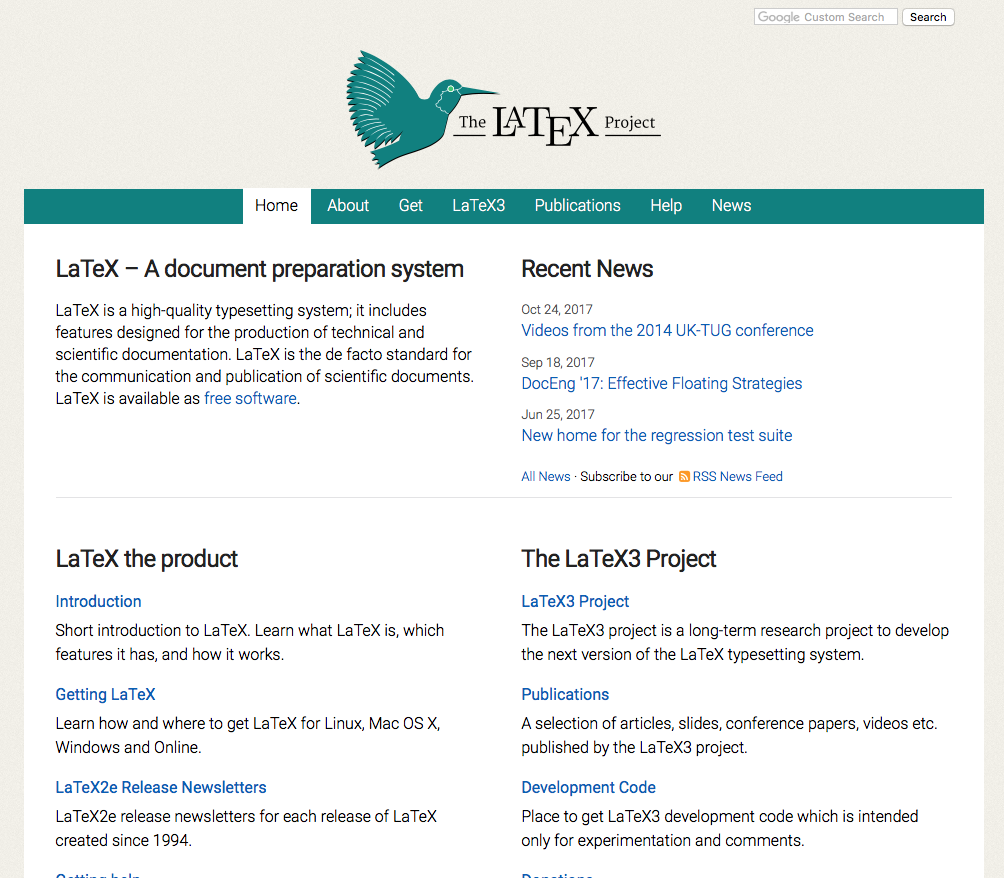
\includegraphics[width=0.7\textwidth]{figures/fig_latex_project_org}
\par\end{centering}

\caption{LaTeX Project}
\end{figure}


Puede obtener, en forma gratuita, las distribuciones de \LaTeX{},
según su plataforma, en:

\begin{description}
\item [Windows] \href{http://miktex.org/}{http://miktex.org/}; también puede
ocupar \href{http://www.tug.org/protext/}{http://www.tug.org/protext/}.

MikTex ofrece una versión básica. Después de instalarlo, asegúrese de descargar los paquetes adicionales requeridos para compilar esta plantilla.

\item [MacOS] \href{http://www.tug.org/mactex/}{http://www.tug.org/mactex/}.

La versión de MacTex es completa e incluye por defecto todos los paquetes necesarios para compilar esta plantilla.

\item [Unix/Linux] \href{http://www.tug.org/texlive/}{http://www.tug.org/texlive/}.

La instalación de TexLive en plataformas *nix es muy sencilla y directa a través de una consola (con permisos de administración):

(K/X)Ubuntu / Debian: \inlinecode{# apt-get install texlive}

Fedora: \inlinecode{# dnf install texlive}

RedHat / CentOS: \inlinecode{# yum install texlive}
\end{description}

Para una referencia completa sobre \LaTeX{}, recomendamos el libro
de \citealp{Lamport94}; aunque para solucionar problemas específicos,
su mejor aliado es Internet. Otros libros que puede consultar se presentan
en la Bibliografía \citep{Mittelbach04,Oetiker06,Roberts05}.


\section{Editores para \LaTeX}
Existen muchos editores de \LaTeX, la mayoría de ellos de distribución gratuita y con versiones para los distintos sistemas operativos:
\begin{description}
    \item [TexStudio] Mac, Windows y Linux. \href{www.texstudio.org}{www.texstudio.org}.
    \item [TexMaker] Mac, Windows y Linux.  \href{www.xm1math.net/texmaker/}{www.xm1math.net/texmaker/}.
    \item[TeXworks] Mac, Window y Linux. \href{https://www.tug.org/texworks/}{https://www.tug.org/texworks/}
    \item [TexShop] Mac. \href{http://pages.uoregon.edu/koch/texshop/}{http://pages.uoregon.edu/koch/texshop/}.
    \item[Kile] Linux y Mac (vía macports). \href{http://kile.sourceforge.net/}{http://kile.sourceforge.net/}.
    \item[LaTeXila] Linux y Mac (vía Homebrew). \href{https://wiki.gnome.org/Apps/LaTeXila\#Installation}{https://wiki.gnome.org/Apps/LaTeXila\#Installation}.
\end{description}

%...              % Agregar aquí más capítulos
\end{Verbatim}

\section{Para tomar en cuenta (Recomendaciones)}

\subsection{Impresión por ambos lados.}
Este documento está preparado para ser impreso por ambos lados de una hoja (\emph{``twoside''}). Para cambiar esto, en la ``clase de documento'', reemplazar la palabra \emph{``twoside''} por \emph{``oneside''}. Es por esto que encontrará algunas hojas que están en blanco, aparentemente sin motivo.


\begin{Verbatim}[frame=lines, label=\inlinecode{memoria.tex} (extracto)
, fontsize=\footnotesize
, baselinestretch=1
, formatcom=\color{gray}]
%---------------------------------------------------------------------------
%%% DOCUMENT CLASS
\documentclass[
    11pt,
    letterpaper,
    twoside
]{thesis_utfsm}
%---------------------------------------------------------------------------
\end{Verbatim}


Es posible que debas cambiar otras configuraciones también para imprimir por un sólo lado. En particular aquellas páginas en blanco después de los agradecimientos y dedicatoria.

\section{Codificación de caracteres.}

Todos los archivos \inlinecode{*.tex} de esta plantilla han sido preparados ocupando la codificación de caracteres por defecto \emph{unicode} (UTF-8). Windows (y algunas versiones de OSX) ocupan otro tipo de codificación (ej. \emph{Windows-1252} o \emph{Mac Roman}).

Si deseas ocupar esta plantilla y encuentras problemas con los caracteres acentuados, entonces puedes optar por una de estas tres alternativas:
\begin{enumerate}[(i)]
    \item cambiar tu editor (TexMaker, TexStudio, TexShop, etc.) para que ocupe UTF-8 como codificación de caracteres por defecto; o
    \item cambiar la codificación de cada documento \inlinecode{*.tex} para que ocupe la codificación nativa de tu sistema operativo; y, modifica la configuración (\inlinecode{config.tex}) dice:
    
    \inlinecode{\\usepackage[utf8x]\{inputenc\}}, por el texto \inlinecode{\\usepackage[latin1]\{inputenc\}}.
    \item escribir todo ocupando caracteres pre-acentuados (ej. \inlinecode{\\'a} en lugar de á).
\end{enumerate}

\vspace{10mm}
\begin{framed}
    \textbf{Recuerda:} Mezclar documentos de distintas codificaciones puede generarte muchos problemas al momento de compilar.  
\end{framed}


\section{Requisitos}
Los paquetes que se ocupan y son indispensables para la generación este documento están contenidos en el documento de clase \inlinecode{thesis_utfsm.cls}.

Para que funcione correctamente se requiere tener instaladas (como mínimo) las siguientes extensiones \LaTeX{}:
\begin{Verbatim}[frame=lines, label=Paquetes requeridos por \inlinecode{thesis_utfsm.sty}
				, fontsize=\footnotesize
				, baselinestretch=1
				, formatcom=\color{gray}]
geometry    % Márgenes y tamaño de páginas
natbib      % Bibliografía
fontenc     % Codificación de Caracteres
inputenc    % Métodos de entrada (acentos)
fancyhdr    % Encabezados 'Fancy'
chngcntr    % Formatos de Pie de Página
booktabs    % Tablas
tabularx    % Tablas
multirow    % Tablas con multi-columnas / multi-filas
array       % Matrices
float       % Imágenes Flotantes
textcomp    % Símbolos de uso común
endnotes    % Notas finales del documento
paralist    % Mejores Listados
listings    % Mejores Listados
framed      % Marcos
fancybox    % Marcos 'Fancy'
verbatim    % Código Fuente
fancyvrb    % Código Fuente 'Fancy'
wrapfig     % Figuras flotantes
xcolor      % Colores personalizados
graphix     % Mejor inclusión de figuras
subfig      % Figuras con múltiples leyendas
tikz        % Diagramas vectoriales
caption     % Mejores leyendas para figuras y tablas
tocbibind   % Bibliografía en la Tabla de Contenidos
rotating    % Rotación de Tablas
asmmath     % Notación ciéntifica / matemática
asmsymb     % Símbolos matemáticos y letras griegas
txfonts     % Times New Roman (para sistemas distintos de Windows)
microtype   % Mejoras subliminales en el uso de fuentes
parskip     % Separación entre párrafos
\end{Verbatim}

La mayoría de las distribuciones \LaTeX{} traen estos paquetes por defecto, sin embargo, en Windows es posible que deba instalar algunos de ellos si ha instalado el archivo básico de MikTeX.



%%%%%
\section{Diagramación}
Este documento fue realizado usando \LaTeX{} (\citeauthor{latex:whatis}), aunque puede fácilmente ser exportado a LyX (\citeauthor{lyx}). Para ver como transformarlo a Lyx, puede revisar el Wiki (\citeauthor{wikilyx}).

Usted necesitará un compilador de \LaTeX. Los más comúnmente ocupados son \citeauthor{miktex} (Windows) y \citeauthor{mactex} (Apple); Sistemas *nix (incluyendo linux) traen \TeX{} por defecto.

Para una referencia completa sobre \LaTeX{}, recomendamos el libro de \cite{Lamport94}; aunque para solucionar problemas específicos, su mejor aliado es Internet.

% Other Author (Included only in Bibliography)
También puede revisar \citet{Roberts05}, \citet{Oetiker06}, y \citet{Mittelbach04}.

\subsection{Figuras}
La siguiente es una figura basada en el archivo \inlinecode{figures/logoind.png}. En este caso, la descripción de la figura va en la parte inferior (ver \autoref{fig:logoind2}).

% Inclusión de Figuras
\begin{figure}[ht!]
\centering

\includegraphics[width=.4\textwidth]{figures/logoind.png}
\caption[Logotipo Departamento de Industrias]{Logotipo Departamento de Industrias\\
{\scriptsize (Fuente: Departamento de Industrias)}}
\label{fig:logoind2}
\end{figure}

La forma de incorporar la \autoref{fig:logoind2} se muestra a continuación:


\begin{Verbatim}[frame=lines, label=Incorporar \autoref{fig:logoind2}
				, fontsize=\footnotesize, numbers=left
				, baselinestretch=1
				, formatcom=\color{gray}]
\begin{figure}[h]
\centering

\includegraphics[width=.4\textwidth]{figures/logoind.png}
\caption[Logotipo Departamento de Industrias]{Logotipo Departamento de Industrias\\
{\scriptsize (Fuente: Departamento de Industrias)}}
\label{fig:logoind2}
\end{figure}
\end{Verbatim}

Otra forma de incorporar figuras es mediante un \inlinecode{float}. En este caso, la figura es incorporada como una imagen ``flotante'' a un costado del texto  (ver Figura \autoref{fig:logousm_float}).

\begin{wrapfigure}{o}{.4\textwidth}
    \vspace{-20pt}
    \begin{spacing}{1}
        \begin{center}
            
\includegraphics[width=.35\columnwidth]{figures/logousm.png}
            \vspace{-10pt}
            \caption{Logotipo USM (Float)}
            \label{fig:logousm_float}
        \end{center}
    \end{spacing}
    \vspace{-10pt}
\end{wrapfigure}

Lorem ipsum dolor sit amet, consectetuer adipiscing elit. Ut purus elit, vestibulum ut, placerat ac, adipiscing vitae, felis. Curabitur dictum gravida mauris. Nam arcu libero, nonummy eget, consectetuer id, vulputate a, magna. Donec vehicula augue eu neque. Pellentesque habitant morbi tristique senectus et netus et malesuada fames ac turpis egestas. Mauris ut leo. Cras viverra metus rhoncus sem. Nulla et lectus vestibulum urna fringilla ultrices. Phasellus eu tellus sit amet tortor gravida placerat. Integer sapien est, iaculis in, pretium quis, viverra ac, nunc. Praesent eget sem vel leo ultrices bibendum. Aenean faucibus. Morbi dolor nulla, malesuada eu, pulvinar at, mollis ac, nulla. Curabitur auctor semper nulla. Donec varius orci eget risus. Duis nibh mi, congue eu, accumsan eleifend, sagittis quis, diam. Duis eget orci sit amet orci dignissim rutrum.



\begin{Verbatim}[frame=lines, label=\autoref{fig:logousm_float}
				, fontsize=\footnotesize, numbers=left
				, baselinestretch=1
				, formatcom=\color{gray}]
\begin{wrapfigure}{o}{.4\textwidth}
    \vspace{-20pt}
    \begin{spacing}{1}
        \begin{center}
            
\includegraphics[width=.35\columnwidth]{figures/logousm.png}
            \vspace{-10pt}
            \caption{Logotipo USM (Float)}
            \label{fig:logousm_float}
        \end{center}
    \end{spacing}
    \vspace{-10pt}
\end{wrapfigure}
\end{Verbatim}


\subsection{Tablas}

La siguiente es una tabla o cuadro básica (ver \autoref{tbl:temperaturas}). Notar las referencias cruzadas y el título de la tabla en la parte superior.

\begin{table}[h!]
    \caption{Tabla de Temperaturas}\label{tbl:temperaturas}
    \begin{tabularx}{\linewidth}{  l  c  c  X }
    \hline
    \textbf{\textsc{Day}} &  \textbf{\textsc{Min Temp}} 
    		& \textbf{\textsc{Max Temp}} & \textbf{\textsc{Summary}}\\
	  \hline\hline
    Monday & 11C & 22C & A clear day with lots of sunshine.
    However, the strong breeze will bring down the temperatures. \\ \hline
    Tuesday & 9C & 19C & Cloudy with rain, across many northern regions. Clear spells
    across most of Scotland and Northern Ireland,
    but rain reaching the far northwest. \\ \hline
    Wednesday & 10C & 21C & Rain will still linger for the morning.
    Conditions will improve by early afternoon and continue
    throughout the evening. \\
    \hline
    \end{tabularx}
\end{table}

\begin{Verbatim}[frame=lines, label=\autoref{fig:logousm_float}
				, fontsize=\footnotesize, numbers=left
				, baselinestretch=1
				, formatcom=\color{gray}]
\begin{table}[h!]
    \caption{Tabla de Temperaturas}\label{tbl:temperaturas}
    \begin{tabularx}{\linewidth}{  l  c  c  X }
    \hline
    \textbf{\textsc{Day}} &  \textbf{\textsc{Min Temp}} 
    		& \textbf{\textsc{Max Temp}} & \textbf{\textsc{Summary}}\\
	  \hline\hline
    Monday & 11C & 22C & A clear day with lots of sunshine.
    However, the strong breeze will bring down the temperatures. \\ \hline
    Tuesday & 9C & 19C & Cloudy with rain, across many northern regions. Clear spells
    across most of Scotland and Northern Ireland,
    but rain reaching the far northwest. \\ \hline
    Wednesday & 10C & 21C & Rain will still linger for the morning.
    Conditions will improve by early afternoon and continue
    throughout the evening. \\
    \hline
    \end{tabularx}
\end{table}
\end{Verbatim}



\subsubsection{Rotación de Tablas}
En caso de tener tablas muy grandes, o si necesita una tabla rotada.
\begin{sidewaystable}
    \centering
    \caption{Rotación de Tablas}
    \begin{tabularx}{\columnwidth}{X X}
        \hline\hline
        \textbf{Column 1} & \textbf{Column 2}\\
        \hline
        Second First & Second Second\\
        \blindtext & \blindtext\\
        \hline\hline
    \end{tabularx}
\end{sidewaystable}


\newpage

\subsection{Opciones Avanzadas para Gráficos}

Los packetes Ti\emph{k}Z y PGF ofrecen alternativas para la creación de gráficos con las más diversas formas y opciones. Para ver opciones consultar \href{http://www.texample.net/tikz/}{www.texample.net/tikz/}.


\newcommand{\MonetaryLevel}{Monetary level}
\newcommand{\RealLevel}{Real level}
\newcommand{\Firms}{Firms}
\newcommand{\Households}{Households}
\newcommand{\Banks}{Banks}
\newcommand{\Commodities}{Commodities}
\newcommand{\LaborPower}{Labor power}
\newcommand{\Wages}{Wages}
\newcommand{\Consumption}{Consumption}
\newcommand{\Credits}{Credits}
\newcommand{\Withdrawals}{Withdrawals}
\newcommand{\Deposits}{Deposits}
\newcommand{\Repayments}{Repayments}

\newcommand{\yslant}{0.5}
\newcommand{\xslant}{-0.6}

\begin{figure}[H]
\centering
\begin{tikzpicture}[scale=1,every node/.style={minimum size=1cm},on grid]

	% Real level
	\begin{scope}[
		yshift=-120,
		every node/.append style={yslant=\yslant,xslant=\xslant},
		yslant=\yslant,xslant=\xslant
	] 
		% The frame:
		\draw[black, dashed, thin] (0,0) rectangle (7,7); 
		% Agents:
		\draw[fill=red]  
			(5,2) circle (.1) % Firms
			(2,2) circle (.1); % Households
		% Flows:
		\draw[-latex,thin] 
			(2,1.8) to[out=-90,in=-90] (5,1.8); % Labour Powers
		\draw[-latex,thin]
			(5,2.2) to[out=90,in=90] (2,2.2); % Wages
		 % Labels:
		\fill[black]
			(0.5,6.5) node[right, scale=.7] {\RealLevel}	
			(5.1,1.9) node[right,scale=.7]{\textbf{\Firms}}
			(1.9,1.9) node[left,scale=.7]{\textbf{\Households}}
			(2.2,3) node [scale=.6, rotate=40] {\Commodities} 
			(4.8,1) node [scale=.6, rotate=40] {\LaborPower};	
	\end{scope}
	
	% 2 vertical lines for linking agents on the 2 levels
	\draw[ultra thin](3.8,4) to (3.8,-0.32);
	\draw[ultra thin](.8,2.4) to (.8,-1.8);
	
	% Monetary level
	\begin{scope}[
		yshift=0,
		every node/.append style={yslant=\yslant,xslant=\xslant},
		yslant=\yslant,xslant=\xslant
	]
		% The frame:
		\fill[white,fill opacity=.75] (0,0) rectangle (7,7); % Opacity
		\draw[black, dashed, thin] (0,0) rectangle (7,7); 
		 % Agents:
		\draw [fill=red]
			(5,2) circle (.1) % Firms
			(2,2) circle (.1) % Households
			(3.5,5) circle (.1); % Banks
		 % Monetary Flows:
		\draw[-latex, thin]
			(3.65,5.1) to[out=30,in=30] (5.15,2.1); % Credits
		\draw[-latex, thin]
			(5,1.8) to[out=-90,in=-90] (2,1.8); % Wages
		\draw[-latex, thin]
			(1.9,2.1) to[out=150,in=150] (3.4,5.1);  % Deposits
		\draw[-latex, thin]
			(3.6,4.9) to[out=-30,in=-30] (2.1,1.9); % Withdrawals
		\draw[-latex, thin]
			(2,2.2) to[out=90,in=90] (5,2.2); % Consumption
		\draw[-latex, thin]
			(4.85,1.9) to[out=210,in=210] (3.35,4.9) ; % Repayments
		 % Labels:
		\fill[black]
			(0.5,6.5) node[right, scale=.7] {\MonetaryLevel}
			(5.1,1.9) node[right,scale=.7]{\textbf {\Firms}}
			(1.9,1.9) node[left,scale=.7]{\textbf {\Households}}
			(3.5,5.1) node[above,scale=.7]{\textbf {\Banks}}
			(5.5,2.8) node [above, scale=.6, rotate=-100] {\Credits}
			(2.6,1.3) node [above, scale=.6, rotate=-10] {\Withdrawals}
			(2.9,4.25) node [above, scale=.6, rotate=50] {\Repayments}
			(2.6,5) node [above, scale=.6, rotate=25] {\Deposits}
			(4.7,2.9) node [above, scale=.6, rotate=-60] {\Consumption}
			(2.3,1.3) node [below, scale=.6, rotate=-40] {\Wages}; 
	\end{scope} 
\end{tikzpicture}
\caption[Gráficos Avanzados con Tikz]{Gráficos Avanzados con Tikz\\ {\scriptsize (Fuente: \url{www.texample.net})}}
\label{fig:tikz}
\end{figure}


\begin{figure}[ht!]
\centering
\usetikzlibrary{chains,fit,shapes}
\begin{tikzpicture}
\tikzstyle{every path}=[very thick]

\edef\sizetape{0.7cm}
\tikzstyle{tmtape}=[draw,minimum size=\sizetape]
\tikzstyle{tmhead}=[arrow box,draw,minimum size=.5cm,arrow box
arrows={east:.25cm, west:0.25cm}]

%% Draw TM tape
\begin{scope}[start chain=1 going right,node distance=-0.15mm]
    \node [on chain=1,tmtape,draw=none] {$\ldots$};
    \node [on chain=1,tmtape] {};
    \node [on chain=1,tmtape] (input) {b};
    \node [on chain=1,tmtape] {b};
    \node [on chain=1,tmtape] {a};
    \node [on chain=1,tmtape] {a};
    \node [on chain=1,tmtape] {a};
    \node [on chain=1,tmtape] {a};
    \node [on chain=1,tmtape] {};
    \node [on chain=1,tmtape,draw=none] {$\ldots$};
    \node [on chain=1] {\textbf{Input/Output Tape}};
\end{scope}

%% Draw TM Finite Control
\begin{scope}
[shift={(3cm,-5cm)},start chain=circle placed {at=(-\tikzchaincount*60:1.5)}]
\foreach \i in {q_0,q_1,q_2,q_3,\ddots,q_n}
	\node [on chain] {$\i$};

% Arrow to current state
\node (center) {};
\draw[->] (center) -- (circle-2);

\node[rounded corners,draw=black,thick,fit=(circle-1) (circle-2) (circle-3) 
      (circle-4) (circle-5) (circle-6),
			label=below:\textbf{Finite Control}] (fsbox)
		{};
\end{scope}

%% Draw TM head below (input) tape cell
\node [tmhead,yshift=-.3cm] at (input.south) (head) {$q_1$};

%% Link Finite Control with Head
\path[->,draw] (fsbox.north) .. controls (4.5,-1) and (0,-2) .. node[right] 
			(headlinetext)
 			{} 
			(head.south);
\node[xshift=3cm] at (headlinetext)  
			{\begin{tabular}{c} 
				\textbf{Reading and Writing Head} \\  
				\textbf{(moves in both directions)} 
			 \end{tabular}};

\end{tikzpicture}
\caption [Diagrama de la Máquina de Türing]{Diagrama de la Máquina de Türing\\ {\scriptsize (Fuente: \url{www.texample.net})}}
\end{figure}


\begin{figure}[ht!]
\centering
% Styles
\tikzstyle{load}   = [ultra thick,-latex]
\tikzstyle{stress} = [-latex]
\tikzstyle{dim}    = [latex-latex]
\tikzstyle{axis}   = [-latex,black!55]

% Drawing Views
\tikzstyle{isometric}=[x={(0.710cm,-0.410cm)},y={(0cm,0.820cm)},z={(-0.710cm,-0.410cm)}]
\tikzstyle{dimetric} =[x={(0.935cm,-0.118cm)},y={(0cm,0.943cm)},z={(-0.354cm,-0.312cm)}]
\tikzstyle{dimetric2}=[x={(0.935cm,-0.118cm)},z={(0cm,0.943cm)},y={(+0.354cm,+0.312cm)}]
\tikzstyle{trimetric}=[x={(0.926cm,-0.207cm)},y={(0cm,0.837cm)},z={(-0.378cm,-0.507cm)}]

  \begin{tikzpicture}[scale=.8]
    \node (origin) at (0,0) {}; % shift relative baseline
    \coordinate (O) at (2,3);
    \draw[fill=gray!10] (O) circle (1);
    \draw[fill=white] (O) circle (0.75) node[below,yshift=-1.125cm] {Signpost Cross Section};
    \draw[dim] (O) ++(-0.75,0) -- ++(1.5,0) node[midway,above] {$d_i$};
    \draw[dim] (O) ++(-1,1.25) -- ++(2,0) node[midway,above] {$d_o$}; 
    \foreach \x in {-1,1} {
      \draw (O) ++(\x,0.25) -- ++(0,1.25);
    }
  \end{tikzpicture}%
  \begin{tikzpicture}[dimetric2]
        \coordinate (O) at (0,0,0);
        \draw[axis] (O) -- ++(6,0,0) node[right] {$x$};
        \draw[axis] (O) -- ++(0,6,0) node[above right] {$y$};
        \draw[axis] (O) -- ++(0,0,6) node[above] {$z$};
        \draw[fill=gray!50] (0,0,-0.5) circle (0.5); 
        \fill[fill=gray!50] (-0.46,-0.2,-0.5) -- (0.46,0.2,-0.5) -- (0.46,0.2,0) -- (-0.46,-0.2,0) -- cycle;
        \draw[fill=gray!20] (O) circle (0.5);
    \draw (0.46,0.2,-0.5) -- ++(0,0,0.5) node[below right,pos=0.0] {Fixed Support};
    \draw (-0.46,-0.2,-0.5) -- ++(0,0,0.5);
    \draw[fill=gray!10] (O) circle (0.2);
    \fill[fill=gray!10] (-0.175,-0.1,0) -- (0.175,0.1,0) -- ++(0,0,4) -- (-0.175,-0.1,4) -- cycle;
    \draw (-0.175,-0.1,0) -- ++(0,0,4);
    \draw (0.175,0.1,0) -- ++(0,0,4) node[right,midway] {Steel Post};
    \draw (4,0,3.95) -- ++(0,0,-1);
    \foreach \z in {0.5,0.75,...,5} {
      \draw[-latex] (-2*\z/5-0.2,0,\z) -- (-0.2,0,\z);
    }
    \draw[load] (0,0,4) -- ++(0,0,-1.25) node[right,xshift=0.1cm] {$F_{z1}$};
    \draw[fill=gray!20] (-0.25,-0.25,5) -- (4,-0.25,5) -- (4,+0.25,5) -- (-0.25,+0.25,5) -- cycle; 
    \draw[fill=gray!50] (+4.00,-0.25,4) -- (4,+0.25,4) -- (4,+0.25,5) -- (+4.00,-0.25,5) -- cycle; 
    \draw[fill=gray!10] (-0.25,-0.25,4) -- (4,-0.25,4) -- (4,-0.25,5) -- (-0.25,-0.25,5) -- cycle; 
    \draw (4.05,0,4) -- ++(1,0,0);
    \draw (4.05,0,5) -- ++(1,0,0);
    \draw[dim] (4.5,0,0) -- ++(0,0,4) node[midway,right] {$h_1$};
    \draw[dim] (4.5,0,4) -- ++(0,0,1) node[midway,right] {$h_2$};
    \draw[dim] (0,0,3.4) -- ++(4,0,0) node[midway,below] {$b_2$};
    \coordinate (P) at (2,-0.25,4.5);
    \draw (P) -- ++(0,0,0.25);
    \draw (P) -- ++(0.25,0,0);
    \draw[dim] (2.125,-0.25,4.5) -- ++(0,0,-0.5) node[midway,right] {$z_1$};
    \draw[dim] (2,-0.25,4.625) -- ++(-2,0,0) node[midway,below] {$x_1$};
    \draw[load] (2,-2.45,4.5) -- ++(0,2.2,0) node[pos=0.0,right,xshift=0.08cm] {$F_{y1}$};
    \draw[axis,dashed,-] (O) -- (0,0,5);
    \draw (0,0,5.5) -- ++(4,0,0) node[midway,above] {$w_{z}$};
    \foreach \x in {0,0.25,...,4} {
      \draw[-latex] (\x,0,5.5) -- ++(0,0,-0.5);
    }
    \draw (-0.2,0,0) -- ++(-2,0,5) node[above,xshift=0.5cm] {$w_{x}=\frac{z}{h_1+h_2} w_0$};
  \end{tikzpicture} 
  \caption [Cargas aplicadas sobre un poste.]{Cargas aplicadas sobre un poste.\\ {\scriptsize (Fuente: \url{www.texample.net})}}
\end{figure}




%!TEX root = memoria.tex

\chapter{¿Cómo usar esta Plantilla?}

Para instrucciones sobre el uso y configuración de esta plantilla, por favor, revise el documento \inlinecode{/latex/memoria.tex} con un editor de texto o editor de \LaTeX{}.

Toda configuración general se encuentra en el documento maestro (\inlinecode{/latex/memoria.tex}). Ahí podrá cambiar los parámetros de la portada y los documentos a incluir. Por ejemplo, si necesita más capítulos, simplemente puede agregarlos creando el archivo (ej. \inlinecode{/latex/chap03.tex}) e incorporando la siguiente línea en el documento maestro:

\inlinecode{\\input\{chap03\}}

\begin{Verbatim}[frame=lines, label=\inlinecode{/latex/memoria.tex} (extracto)
				, fontsize=\footnotesize
				, baselinestretch=1
				, formatcom=\color{gray}]
%%%%%%%%%%%%%%%%%%%%%%%%%%%%%%%%%%%%%
%	Cuerpo Principal (Main Matter)
%%%%%%%%%%%%%%%%%%%%%%%%%%%%%%%%%%%%%
\mainmatter
\pagestyle{fancy}

\input{chap1}			% Archivo chap1.tex
\input{chap2}			% Archivo chap2.tex
\input{chap3}			% Archivo chap3.tex
%...              % Agregar aquí más capítulos
\end{Verbatim}


Además se muestran a continuación ejemplos básicos para la inclusión de figuras y tablas (según formatos exigidos por la UTFSM).

\section{Requerimientos}
Los formatos para la generación este documento están contenidos en la Hoja de Estilo \inlinecode{/memoriaUSM.sty}, que afecta tanto a plantillas \LaTeX{} como LyX.

Para que funcione correctamente se requiere tener instaladas las siguientes extensiones \LaTeX{}:
\begin{Verbatim}[frame=lines, label=Paquetes requeridos por \inlinecode{/memoriaUSM.sty}
				, fontsize=\footnotesize
				, baselinestretch=1
				, formatcom=\color{gray}]
geometry    % Márgenes y tamaño de páginas
natbib      % Bibliografía
fontenc     % Codificación de Caracteres
inputenc    % Métodos de entrada (acentos)
fancyhdr    % Encabezados 'Fancy'
chngcntr    % Formatos de Pie de Página
booktabs    % Tablas
tabularx    % Tablas
multirow    % Tablas con multi-columnas / multi-filas
array       % Matrices
float       % Imágenes Flotantes
textcomp    % Símbolos de uso común
endnotes    % Notas finales del documento
paralist    % Mejores Listados
listings    % Mejores Listados
framed      % Marcos
fancybox    % Marcos 'Fancy'
verbatim    % Código Fuente
fancyvrb    % Código Fuente 'Fancy'
wrapfig     % Figuras flotantes
xcolor      % Colores personalizados
graphix     % Mejor inclusión de figuras
subfig      % Figuras con múltiples leyendas
tikz        % Diagramas vectoriales
caption     % Mejores leyendas para figuras y tablas
tocbibind   % Bibliografía en la Tabla de Contenidos
rotating    % Rotación de Tablas
asmmath     % Notación ciéntifica / matemática
asmsymb     % Símbolos matemáticos y letras griegas
txfonts     % Times New Roman (para sistemas distintos de Windows)
microtype   % Mejoras subliminales en el uso de fuentes
parskip     % Separación entre párrafos
\end{Verbatim}

La mayoría de las distribuciones \LaTeX{} traen estos paquetes por defecto, sin embargo, en Windows es posible que deba instalar algunos de ellos si ha instalado el archivo básico de MikTeX.

\section{Figuras}
La siguiente es una figura basada en el archivo \inlinecode{/latex/figures/logoind.png}. En este caso, la descripción de la figura va en la parte inferior (ver \autoref{fig:logoind2}).

% Inclusión de Figuras
\begin{figure}[ht!]
\centering

\includegraphics[width=.4\textwidth]{figures/logoind.png}
\caption[Logotipo Departamento de Industrias]{Logotipo Departamento de Industrias\\
{\scriptsize (Fuente: Departamento de Industrias)}}
\label{fig:logoind2}
\end{figure}

La forma de incorporar la \autoref{fig:logoind2} se muestra a continuación:


\begin{Verbatim}[frame=lines, label=Incorporar \autoref{fig:logoind2}
				, fontsize=\footnotesize, numbers=left
				, baselinestretch=1
				, formatcom=\color{gray}]
\begin{figure}[h]
\centering

\includegraphics[width=.4\textwidth]{figures/logoind.png}
\caption[Logotipo Departamento de Industrias]{Logotipo Departamento de Industrias\\
{\scriptsize (Fuente: Departamento de Industrias)}}
\label{fig:logoind2}
\end{figure}
\end{Verbatim}

Otra forma de incorporar figuras es mediante un \inlinecode{float}. En este caso, la figura es incorporada como una imagen ``flotante'' a un costado del texto  (ver Figura \autoref{fig:logousm_float}).

\begin{wrapfigure}{o}{.4\textwidth}
    \vspace{-20pt}
    \begin{spacing}{1}
        \begin{center}
            
\includegraphics[width=.35\columnwidth]{figures/logousm.png}
            \vspace{-10pt}
            \caption{Logotipo USM (Float)}
            \label{fig:logousm_float}
        \end{center}
    \end{spacing}
    \vspace{-10pt}
\end{wrapfigure}

Lorem ipsum dolor sit amet, consectetuer adipiscing elit. Ut purus elit, vestibulum ut, placerat ac, adipiscing vitae, felis. Curabitur dictum gravida mauris. Nam arcu libero, nonummy eget, consectetuer id, vulputate a, magna. Donec vehicula augue eu neque. Pellentesque habitant morbi tristique senectus et netus et malesuada fames ac turpis egestas. Mauris ut leo. Cras viverra metus rhoncus sem. Nulla et lectus vestibulum urna fringilla ultrices. Phasellus eu tellus sit amet tortor gravida placerat. Integer sapien est, iaculis in, pretium quis, viverra ac, nunc. Praesent eget sem vel leo ultrices bibendum. Aenean faucibus. Morbi dolor nulla, malesuada eu, pulvinar at, mollis ac, nulla. Curabitur auctor semper nulla. Donec varius orci eget risus. Duis nibh mi, congue eu, accumsan eleifend, sagittis quis, diam. Duis eget orci sit amet orci dignissim rutrum.



\begin{Verbatim}[frame=lines, label=\autoref{fig:logousm_float}
				, fontsize=\footnotesize, numbers=left
				, baselinestretch=1
				, formatcom=\color{gray}]
\begin{wrapfigure}{o}{.4\textwidth}
    \vspace{-20pt}
    \begin{spacing}{1}
        \begin{center}
            
\includegraphics[width=.35\columnwidth]{figures/logousm.png}
            \vspace{-10pt}
            \caption{Logotipo USM (Float)}
            \label{fig:logousm_float}
        \end{center}
    \end{spacing}
    \vspace{-10pt}
\end{wrapfigure}
\end{Verbatim}


\section{Tablas}

La siguiente es una tabla o cuadro básica (ver \autoref{tbl:temperaturas}). Notar las referencias cruzadas y el título de la tabla en la parte superior.

\begin{table}[h!]
    \caption{Tabla de Temperaturas}\label{tbl:temperaturas}
    \begin{tabularx}{\linewidth}{  l  c  c  X }
    \hline
    \textbf{\textsc{Day}} &  \textbf{\textsc{Min Temp}} 
    		& \textbf{\textsc{Max Temp}} & \textbf{\textsc{Summary}}\\
	  \hline\hline
    Monday & 11C & 22C & A clear day with lots of sunshine.
    However, the strong breeze will bring down the temperatures. \\ \hline
    Tuesday & 9C & 19C & Cloudy with rain, across many northern regions. Clear spells
    across most of Scotland and Northern Ireland,
    but rain reaching the far northwest. \\ \hline
    Wednesday & 10C & 21C & Rain will still linger for the morning.
    Conditions will improve by early afternoon and continue
    throughout the evening. \\
    \hline
    \end{tabularx}
\end{table}

\begin{Verbatim}[frame=lines, label=\autoref{fig:logousm_float}
				, fontsize=\footnotesize, numbers=left
				, baselinestretch=1
				, formatcom=\color{gray}]
\begin{table}[h!]
    \caption{Tabla de Temperaturas}\label{tbl:temperaturas}
    \begin{tabularx}{\linewidth}{  l  c  c  X }
    \hline
    \textbf{\textsc{Day}} &  \textbf{\textsc{Min Temp}} 
    		& \textbf{\textsc{Max Temp}} & \textbf{\textsc{Summary}}\\
	  \hline\hline
    Monday & 11C & 22C & A clear day with lots of sunshine.
    However, the strong breeze will bring down the temperatures. \\ \hline
    Tuesday & 9C & 19C & Cloudy with rain, across many northern regions. Clear spells
    across most of Scotland and Northern Ireland,
    but rain reaching the far northwest. \\ \hline
    Wednesday & 10C & 21C & Rain will still linger for the morning.
    Conditions will improve by early afternoon and continue
    throughout the evening. \\
    \hline
    \end{tabularx}
\end{table}
\end{Verbatim}


\section{Opciones Avanzadas para Gráficos}

Los packetes Ti\emph{k}Z y PGF ofrecen alternativas para la creación de gráficos con las más diversas formas y opciones. Para ver opciones consultar \href{http://www.texample.net/tikz/}{www.texample.net/tikz/}.


\newcommand{\MonetaryLevel}{Monetary level}
\newcommand{\RealLevel}{Real level}
\newcommand{\Firms}{Firms}
\newcommand{\Households}{Households}
\newcommand{\Banks}{Banks}
\newcommand{\Commodities}{Commodities}
\newcommand{\LaborPower}{Labor power}
\newcommand{\Wages}{Wages}
\newcommand{\Consumption}{Consumption}
\newcommand{\Credits}{Credits}
\newcommand{\Withdrawals}{Withdrawals}
\newcommand{\Deposits}{Deposits}
\newcommand{\Repayments}{Repayments}

\newcommand{\yslant}{0.5}
\newcommand{\xslant}{-0.6}

\begin{figure}[H]
\centering
\begin{tikzpicture}[scale=1,every node/.style={minimum size=1cm},on grid]

	% Real level
	\begin{scope}[
		yshift=-120,
		every node/.append style={yslant=\yslant,xslant=\xslant},
		yslant=\yslant,xslant=\xslant
	] 
		% The frame:
		\draw[black, dashed, thin] (0,0) rectangle (7,7); 
		% Agents:
		\draw[fill=red]  
			(5,2) circle (.1) % Firms
			(2,2) circle (.1); % Households
		% Flows:
		\draw[-latex,thin] 
			(2,1.8) to[out=-90,in=-90] (5,1.8); % Labour Powers
		\draw[-latex,thin]
			(5,2.2) to[out=90,in=90] (2,2.2); % Wages
		 % Labels:
		\fill[black]
			(0.5,6.5) node[right, scale=.7] {\RealLevel}	
			(5.1,1.9) node[right,scale=.7]{\textbf{\Firms}}
			(1.9,1.9) node[left,scale=.7]{\textbf{\Households}}
			(2.2,3) node [scale=.6, rotate=40] {\Commodities} 
			(4.8,1) node [scale=.6, rotate=40] {\LaborPower};	
	\end{scope}
	
	% 2 vertical lines for linking agents on the 2 levels
	\draw[ultra thin](3.8,4) to (3.8,-0.32);
	\draw[ultra thin](.8,2.4) to (.8,-1.8);
	
	% Monetary level
	\begin{scope}[
		yshift=0,
		every node/.append style={yslant=\yslant,xslant=\xslant},
		yslant=\yslant,xslant=\xslant
	]
		% The frame:
		\fill[white,fill opacity=.75] (0,0) rectangle (7,7); % Opacity
		\draw[black, dashed, thin] (0,0) rectangle (7,7); 
		 % Agents:
		\draw [fill=red]
			(5,2) circle (.1) % Firms
			(2,2) circle (.1) % Households
			(3.5,5) circle (.1); % Banks
		 % Monetary Flows:
		\draw[-latex, thin]
			(3.65,5.1) to[out=30,in=30] (5.15,2.1); % Credits
		\draw[-latex, thin]
			(5,1.8) to[out=-90,in=-90] (2,1.8); % Wages
		\draw[-latex, thin]
			(1.9,2.1) to[out=150,in=150] (3.4,5.1);  % Deposits
		\draw[-latex, thin]
			(3.6,4.9) to[out=-30,in=-30] (2.1,1.9); % Withdrawals
		\draw[-latex, thin]
			(2,2.2) to[out=90,in=90] (5,2.2); % Consumption
		\draw[-latex, thin]
			(4.85,1.9) to[out=210,in=210] (3.35,4.9) ; % Repayments
		 % Labels:
		\fill[black]
			(0.5,6.5) node[right, scale=.7] {\MonetaryLevel}
			(5.1,1.9) node[right,scale=.7]{\textbf {\Firms}}
			(1.9,1.9) node[left,scale=.7]{\textbf {\Households}}
			(3.5,5.1) node[above,scale=.7]{\textbf {\Banks}}
			(5.5,2.8) node [above, scale=.6, rotate=-100] {\Credits}
			(2.6,1.3) node [above, scale=.6, rotate=-10] {\Withdrawals}
			(2.9,4.25) node [above, scale=.6, rotate=50] {\Repayments}
			(2.6,5) node [above, scale=.6, rotate=25] {\Deposits}
			(4.7,2.9) node [above, scale=.6, rotate=-60] {\Consumption}
			(2.3,1.3) node [below, scale=.6, rotate=-40] {\Wages}; 
	\end{scope} 
\end{tikzpicture}
\caption[Gráficos Avanzados con Tikz]{Gráficos Avanzados con Tikz\\ {\scriptsize (Fuente: \url{www.texample.net})}}
\label{fig:tikz}
\end{figure}


\begin{figure}[ht!]
\centering
\usetikzlibrary{chains,fit,shapes}
\begin{tikzpicture}
\tikzstyle{every path}=[very thick]

\edef\sizetape{0.7cm}
\tikzstyle{tmtape}=[draw,minimum size=\sizetape]
\tikzstyle{tmhead}=[arrow box,draw,minimum size=.5cm,arrow box
arrows={east:.25cm, west:0.25cm}]

%% Draw TM tape
\begin{scope}[start chain=1 going right,node distance=-0.15mm]
    \node [on chain=1,tmtape,draw=none] {$\ldots$};
    \node [on chain=1,tmtape] {};
    \node [on chain=1,tmtape] (input) {b};
    \node [on chain=1,tmtape] {b};
    \node [on chain=1,tmtape] {a};
    \node [on chain=1,tmtape] {a};
    \node [on chain=1,tmtape] {a};
    \node [on chain=1,tmtape] {a};
    \node [on chain=1,tmtape] {};
    \node [on chain=1,tmtape,draw=none] {$\ldots$};
    \node [on chain=1] {\textbf{Input/Output Tape}};
\end{scope}

%% Draw TM Finite Control
\begin{scope}
[shift={(3cm,-5cm)},start chain=circle placed {at=(-\tikzchaincount*60:1.5)}]
\foreach \i in {q_0,q_1,q_2,q_3,\ddots,q_n}
	\node [on chain] {$\i$};

% Arrow to current state
\node (center) {};
\draw[->] (center) -- (circle-2);

\node[rounded corners,draw=black,thick,fit=(circle-1) (circle-2) (circle-3) 
      (circle-4) (circle-5) (circle-6),
			label=below:\textbf{Finite Control}] (fsbox)
		{};
\end{scope}

%% Draw TM head below (input) tape cell
\node [tmhead,yshift=-.3cm] at (input.south) (head) {$q_1$};

%% Link Finite Control with Head
\path[->,draw] (fsbox.north) .. controls (4.5,-1) and (0,-2) .. node[right] 
			(headlinetext)
 			{} 
			(head.south);
\node[xshift=3cm] at (headlinetext)  
			{\begin{tabular}{c} 
				\textbf{Reading and Writing Head} \\  
				\textbf{(moves in both directions)} 
			 \end{tabular}};

\end{tikzpicture}
\caption [Diagrama de la Máquina de Türing]{Diagrama de la Máquina de Türing\\ {\scriptsize (Fuente: \url{www.texample.net})}}
\end{figure}


\begin{figure}[ht!]
\centering
% Styles
\tikzstyle{load}   = [ultra thick,-latex]
\tikzstyle{stress} = [-latex]
\tikzstyle{dim}    = [latex-latex]
\tikzstyle{axis}   = [-latex,black!55]

% Drawing Views
\tikzstyle{isometric}=[x={(0.710cm,-0.410cm)},y={(0cm,0.820cm)},z={(-0.710cm,-0.410cm)}]
\tikzstyle{dimetric} =[x={(0.935cm,-0.118cm)},y={(0cm,0.943cm)},z={(-0.354cm,-0.312cm)}]
\tikzstyle{dimetric2}=[x={(0.935cm,-0.118cm)},z={(0cm,0.943cm)},y={(+0.354cm,+0.312cm)}]
\tikzstyle{trimetric}=[x={(0.926cm,-0.207cm)},y={(0cm,0.837cm)},z={(-0.378cm,-0.507cm)}]

  \begin{tikzpicture}[scale=.8]
    \node (origin) at (0,0) {}; % shift relative baseline
    \coordinate (O) at (2,3);
    \draw[fill=gray!10] (O) circle (1);
    \draw[fill=white] (O) circle (0.75) node[below,yshift=-1.125cm] {Signpost Cross Section};
    \draw[dim] (O) ++(-0.75,0) -- ++(1.5,0) node[midway,above] {$d_i$};
    \draw[dim] (O) ++(-1,1.25) -- ++(2,0) node[midway,above] {$d_o$}; 
    \foreach \x in {-1,1} {
      \draw (O) ++(\x,0.25) -- ++(0,1.25);
    }
  \end{tikzpicture}%
  \begin{tikzpicture}[dimetric2]
        \coordinate (O) at (0,0,0);
        \draw[axis] (O) -- ++(6,0,0) node[right] {$x$};
        \draw[axis] (O) -- ++(0,6,0) node[above right] {$y$};
        \draw[axis] (O) -- ++(0,0,6) node[above] {$z$};
        \draw[fill=gray!50] (0,0,-0.5) circle (0.5); 
        \fill[fill=gray!50] (-0.46,-0.2,-0.5) -- (0.46,0.2,-0.5) -- (0.46,0.2,0) -- (-0.46,-0.2,0) -- cycle;
        \draw[fill=gray!20] (O) circle (0.5);
    \draw (0.46,0.2,-0.5) -- ++(0,0,0.5) node[below right,pos=0.0] {Fixed Support};
    \draw (-0.46,-0.2,-0.5) -- ++(0,0,0.5);
    \draw[fill=gray!10] (O) circle (0.2);
    \fill[fill=gray!10] (-0.175,-0.1,0) -- (0.175,0.1,0) -- ++(0,0,4) -- (-0.175,-0.1,4) -- cycle;
    \draw (-0.175,-0.1,0) -- ++(0,0,4);
    \draw (0.175,0.1,0) -- ++(0,0,4) node[right,midway] {Steel Post};
    \draw (4,0,3.95) -- ++(0,0,-1);
    \foreach \z in {0.5,0.75,...,5} {
      \draw[-latex] (-2*\z/5-0.2,0,\z) -- (-0.2,0,\z);
    }
    \draw[load] (0,0,4) -- ++(0,0,-1.25) node[right,xshift=0.1cm] {$F_{z1}$};
    \draw[fill=gray!20] (-0.25,-0.25,5) -- (4,-0.25,5) -- (4,+0.25,5) -- (-0.25,+0.25,5) -- cycle; 
    \draw[fill=gray!50] (+4.00,-0.25,4) -- (4,+0.25,4) -- (4,+0.25,5) -- (+4.00,-0.25,5) -- cycle; 
    \draw[fill=gray!10] (-0.25,-0.25,4) -- (4,-0.25,4) -- (4,-0.25,5) -- (-0.25,-0.25,5) -- cycle; 
    \draw (4.05,0,4) -- ++(1,0,0);
    \draw (4.05,0,5) -- ++(1,0,0);
    \draw[dim] (4.5,0,0) -- ++(0,0,4) node[midway,right] {$h_1$};
    \draw[dim] (4.5,0,4) -- ++(0,0,1) node[midway,right] {$h_2$};
    \draw[dim] (0,0,3.4) -- ++(4,0,0) node[midway,below] {$b_2$};
    \coordinate (P) at (2,-0.25,4.5);
    \draw (P) -- ++(0,0,0.25);
    \draw (P) -- ++(0.25,0,0);
    \draw[dim] (2.125,-0.25,4.5) -- ++(0,0,-0.5) node[midway,right] {$z_1$};
    \draw[dim] (2,-0.25,4.625) -- ++(-2,0,0) node[midway,below] {$x_1$};
    \draw[load] (2,-2.45,4.5) -- ++(0,2.2,0) node[pos=0.0,right,xshift=0.08cm] {$F_{y1}$};
    \draw[axis,dashed,-] (O) -- (0,0,5);
    \draw (0,0,5.5) -- ++(4,0,0) node[midway,above] {$w_{z}$};
    \foreach \x in {0,0.25,...,4} {
      \draw[-latex] (\x,0,5.5) -- ++(0,0,-0.5);
    }
    \draw (-0.2,0,0) -- ++(-2,0,5) node[above,xshift=0.5cm] {$w_{x}=\frac{z}{h_1+h_2} w_0$};
  \end{tikzpicture} 
  \caption [Cargas aplicadas sobre un poste.]{Cargas aplicadas sobre un poste.\\ {\scriptsize (Fuente: \url{www.texample.net})}}
\end{figure}




\section{Rotación de Tablas}
En caso de tener tablas muy grandes, o si necesita una tabla rotada.
\begin{sidewaystable}
   \centering
   \caption{Rotación de Tablas}
   \begin{tabularx}{\columnwidth}{X X}
   \hline\hline
    \textbf{Column 1} & \textbf{Column 2}\\
    \hline
    Second First & Second Second\\
    \blindtext & \blindtext\\
    \hline\hline
    \end{tabularx}
\end{sidewaystable}

%!TEX root = ../memoria.tex

\chapter{Instalación de \LaTeX}


\section{\LaTeX}

\LaTeX{} es un sistema de preparación de documentos de alta calidad
visual \citep{latex:whatis}. Si no ha ocupado \LaTeX{} anteriormente,
visite esta página:
\begin{itemize}
\item \href{http://www.latex-project.org/}{http://www.latex-project.org/}
\end{itemize}
\begin{figure}[H]
\begin{centering}
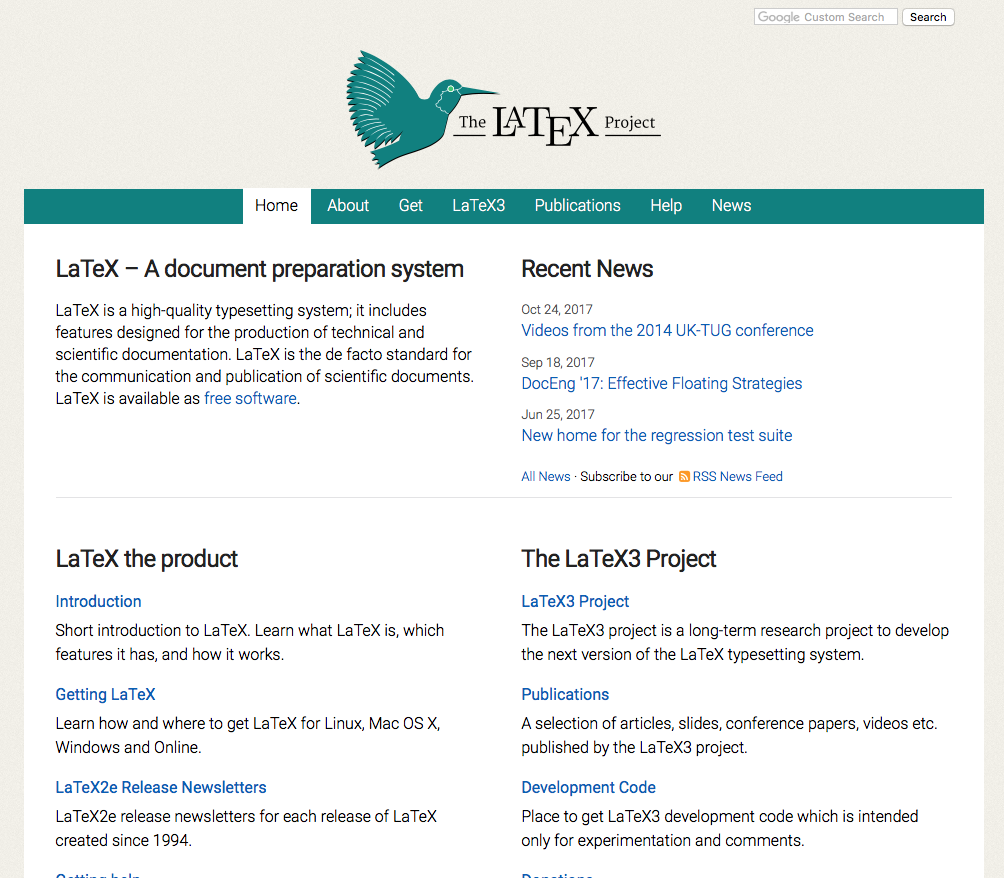
\includegraphics[width=0.7\textwidth]{figures/fig_latex_project_org}
\par\end{centering}

\caption{LaTeX Project}
\end{figure}


Puede obtener, en forma gratuita, las distribuciones de \LaTeX{},
según su plataforma, en:

\begin{description}
\item [Windows] \href{http://miktex.org/}{http://miktex.org/}; también puede
ocupar \href{http://www.tug.org/protext/}{http://www.tug.org/protext/}.

MikTex ofrece una versión básica. Después de instalarlo, asegúrese de descargar los paquetes adicionales requeridos para compilar esta plantilla.

\item [MacOS] \href{http://www.tug.org/mactex/}{http://www.tug.org/mactex/}.

La versión de MacTex es completa e incluye por defecto todos los paquetes necesarios para compilar esta plantilla.

\item [Unix/Linux] \href{http://www.tug.org/texlive/}{http://www.tug.org/texlive/}.

La instalación de TexLive en plataformas *nix es muy sencilla y directa a través de una consola (con permisos de administración):

(K/X)Ubuntu / Debian: \inlinecode{# apt-get install texlive}

Fedora: \inlinecode{# dnf install texlive}

RedHat / CentOS: \inlinecode{# yum install texlive}
\end{description}

Para una referencia completa sobre \LaTeX{}, recomendamos el libro
de \citealp{Lamport94}; aunque para solucionar problemas específicos,
su mejor aliado es Internet. Otros libros que puede consultar se presentan
en la Bibliografía \citep{Mittelbach04,Oetiker06,Roberts05}.


\section{Editores para \LaTeX}
Existen muchos editores de \LaTeX, la mayoría de ellos de distribución gratuita y con versiones para los distintos sistemas operativos:
\begin{description}
    \item [TexStudio] Mac, Windows y Linux. \href{www.texstudio.org}{www.texstudio.org}.
    \item [TexMaker] Mac, Windows y Linux.  \href{www.xm1math.net/texmaker/}{www.xm1math.net/texmaker/}.
    \item[TeXworks] Mac, Window y Linux. \href{https://www.tug.org/texworks/}{https://www.tug.org/texworks/}
    \item [TexShop] Mac. \href{http://pages.uoregon.edu/koch/texshop/}{http://pages.uoregon.edu/koch/texshop/}.
    \item[Kile] Linux y Mac (vía macports). \href{http://kile.sourceforge.net/}{http://kile.sourceforge.net/}.
    \item[LaTeXila] Linux y Mac (vía Homebrew). \href{https://wiki.gnome.org/Apps/LaTeXila\#Installation}{https://wiki.gnome.org/Apps/LaTeXila\#Installation}.
\end{description}

%...              % Agregar aquí más capítulos
\end{Verbatim}

\section{Para tomar en cuenta (Recomendaciones)}

\subsection{Impresión por ambos lados.}
Este documento está preparado para ser impreso por ambos lados de una hoja (\emph{``twoside''}). Para cambiar esto, en la ``clase de documento'', reemplazar la palabra \emph{``twoside''} por \emph{``oneside''}. Es por esto que encontrará algunas hojas que están en blanco, aparentemente sin motivo.


\begin{Verbatim}[frame=lines, label=\inlinecode{memoria.tex} (extracto)
, fontsize=\footnotesize
, baselinestretch=1
, formatcom=\color{gray}]
%---------------------------------------------------------------------------
%%% DOCUMENT CLASS
\documentclass[
    11pt,
    letterpaper,
    twoside
]{thesis_utfsm}
%---------------------------------------------------------------------------
\end{Verbatim}


Es posible que debas cambiar otras configuraciones también para imprimir por un sólo lado. En particular aquellas páginas en blanco después de los agradecimientos y dedicatoria.

\section{Codificación de caracteres.}

Todos los archivos \inlinecode{*.tex} de esta plantilla han sido preparados ocupando la codificación de caracteres por defecto \emph{unicode} (UTF-8). Windows (y algunas versiones de OSX) ocupan otro tipo de codificación (ej. \emph{Windows-1252} o \emph{Mac Roman}).

Si deseas ocupar esta plantilla y encuentras problemas con los caracteres acentuados, entonces puedes optar por una de estas tres alternativas:
\begin{enumerate}[(i)]
    \item cambiar tu editor (TexMaker, TexStudio, TexShop, etc.) para que ocupe UTF-8 como codificación de caracteres por defecto; o
    \item cambiar la codificación de cada documento \inlinecode{*.tex} para que ocupe la codificación nativa de tu sistema operativo; y, modifica la configuración (\inlinecode{config.tex}) dice:
    
    \inlinecode{\\usepackage[utf8x]\{inputenc\}}, por el texto \inlinecode{\\usepackage[latin1]\{inputenc\}}.
    \item escribir todo ocupando caracteres pre-acentuados (ej. \inlinecode{\\'a} en lugar de á).
\end{enumerate}

\vspace{10mm}
\begin{framed}
    \textbf{Recuerda:} Mezclar documentos de distintas codificaciones puede generarte muchos problemas al momento de compilar.  
\end{framed}


\section{Requisitos}
Los paquetes que se ocupan y son indispensables para la generación este documento están contenidos en el documento de clase \inlinecode{thesis_utfsm.cls}.

Para que funcione correctamente se requiere tener instaladas (como mínimo) las siguientes extensiones \LaTeX{}:
\begin{Verbatim}[frame=lines, label=Paquetes requeridos por \inlinecode{thesis_utfsm.sty}
				, fontsize=\footnotesize
				, baselinestretch=1
				, formatcom=\color{gray}]
geometry    % Márgenes y tamaño de páginas
natbib      % Bibliografía
fontenc     % Codificación de Caracteres
inputenc    % Métodos de entrada (acentos)
fancyhdr    % Encabezados 'Fancy'
chngcntr    % Formatos de Pie de Página
booktabs    % Tablas
tabularx    % Tablas
multirow    % Tablas con multi-columnas / multi-filas
array       % Matrices
float       % Imágenes Flotantes
textcomp    % Símbolos de uso común
endnotes    % Notas finales del documento
paralist    % Mejores Listados
listings    % Mejores Listados
framed      % Marcos
fancybox    % Marcos 'Fancy'
verbatim    % Código Fuente
fancyvrb    % Código Fuente 'Fancy'
wrapfig     % Figuras flotantes
xcolor      % Colores personalizados
graphix     % Mejor inclusión de figuras
subfig      % Figuras con múltiples leyendas
tikz        % Diagramas vectoriales
caption     % Mejores leyendas para figuras y tablas
tocbibind   % Bibliografía en la Tabla de Contenidos
rotating    % Rotación de Tablas
asmmath     % Notación ciéntifica / matemática
asmsymb     % Símbolos matemáticos y letras griegas
txfonts     % Times New Roman (para sistemas distintos de Windows)
microtype   % Mejoras subliminales en el uso de fuentes
parskip     % Separación entre párrafos
\end{Verbatim}

La mayoría de las distribuciones \LaTeX{} traen estos paquetes por defecto, sin embargo, en Windows es posible que deba instalar algunos de ellos si ha instalado el archivo básico de MikTeX.



%%%%%
\section{Diagramación}
Este documento fue realizado usando \LaTeX{} (\citeauthor{latex:whatis}), aunque puede fácilmente ser exportado a LyX (\citeauthor{lyx}). Para ver como transformarlo a Lyx, puede revisar el Wiki (\citeauthor{wikilyx}).

Usted necesitará un compilador de \LaTeX. Los más comúnmente ocupados son \citeauthor{miktex} (Windows) y \citeauthor{mactex} (Apple); Sistemas *nix (incluyendo linux) traen \TeX{} por defecto.

Para una referencia completa sobre \LaTeX{}, recomendamos el libro de \cite{Lamport94}; aunque para solucionar problemas específicos, su mejor aliado es Internet.

% Other Author (Included only in Bibliography)
También puede revisar \citet{Roberts05}, \citet{Oetiker06}, y \citet{Mittelbach04}.

\subsection{Figuras}
La siguiente es una figura basada en el archivo \inlinecode{figures/logoind.png}. En este caso, la descripción de la figura va en la parte inferior (ver \autoref{fig:logoind2}).

% Inclusión de Figuras
\begin{figure}[ht!]
\centering

\includegraphics[width=.4\textwidth]{figures/logoind.png}
\caption[Logotipo Departamento de Industrias]{Logotipo Departamento de Industrias\\
{\scriptsize (Fuente: Departamento de Industrias)}}
\label{fig:logoind2}
\end{figure}

La forma de incorporar la \autoref{fig:logoind2} se muestra a continuación:


\begin{Verbatim}[frame=lines, label=Incorporar \autoref{fig:logoind2}
				, fontsize=\footnotesize, numbers=left
				, baselinestretch=1
				, formatcom=\color{gray}]
\begin{figure}[h]
\centering

\includegraphics[width=.4\textwidth]{figures/logoind.png}
\caption[Logotipo Departamento de Industrias]{Logotipo Departamento de Industrias\\
{\scriptsize (Fuente: Departamento de Industrias)}}
\label{fig:logoind2}
\end{figure}
\end{Verbatim}

Otra forma de incorporar figuras es mediante un \inlinecode{float}. En este caso, la figura es incorporada como una imagen ``flotante'' a un costado del texto  (ver Figura \autoref{fig:logousm_float}).

\begin{wrapfigure}{o}{.4\textwidth}
    \vspace{-20pt}
    \begin{spacing}{1}
        \begin{center}
            
\includegraphics[width=.35\columnwidth]{figures/logousm.png}
            \vspace{-10pt}
            \caption{Logotipo USM (Float)}
            \label{fig:logousm_float}
        \end{center}
    \end{spacing}
    \vspace{-10pt}
\end{wrapfigure}

Lorem ipsum dolor sit amet, consectetuer adipiscing elit. Ut purus elit, vestibulum ut, placerat ac, adipiscing vitae, felis. Curabitur dictum gravida mauris. Nam arcu libero, nonummy eget, consectetuer id, vulputate a, magna. Donec vehicula augue eu neque. Pellentesque habitant morbi tristique senectus et netus et malesuada fames ac turpis egestas. Mauris ut leo. Cras viverra metus rhoncus sem. Nulla et lectus vestibulum urna fringilla ultrices. Phasellus eu tellus sit amet tortor gravida placerat. Integer sapien est, iaculis in, pretium quis, viverra ac, nunc. Praesent eget sem vel leo ultrices bibendum. Aenean faucibus. Morbi dolor nulla, malesuada eu, pulvinar at, mollis ac, nulla. Curabitur auctor semper nulla. Donec varius orci eget risus. Duis nibh mi, congue eu, accumsan eleifend, sagittis quis, diam. Duis eget orci sit amet orci dignissim rutrum.



\begin{Verbatim}[frame=lines, label=\autoref{fig:logousm_float}
				, fontsize=\footnotesize, numbers=left
				, baselinestretch=1
				, formatcom=\color{gray}]
\begin{wrapfigure}{o}{.4\textwidth}
    \vspace{-20pt}
    \begin{spacing}{1}
        \begin{center}
            
\includegraphics[width=.35\columnwidth]{figures/logousm.png}
            \vspace{-10pt}
            \caption{Logotipo USM (Float)}
            \label{fig:logousm_float}
        \end{center}
    \end{spacing}
    \vspace{-10pt}
\end{wrapfigure}
\end{Verbatim}


\subsection{Tablas}

La siguiente es una tabla o cuadro básica (ver \autoref{tbl:temperaturas}). Notar las referencias cruzadas y el título de la tabla en la parte superior.

\begin{table}[h!]
    \caption{Tabla de Temperaturas}\label{tbl:temperaturas}
    \begin{tabularx}{\linewidth}{  l  c  c  X }
    \hline
    \textbf{\textsc{Day}} &  \textbf{\textsc{Min Temp}} 
    		& \textbf{\textsc{Max Temp}} & \textbf{\textsc{Summary}}\\
	  \hline\hline
    Monday & 11C & 22C & A clear day with lots of sunshine.
    However, the strong breeze will bring down the temperatures. \\ \hline
    Tuesday & 9C & 19C & Cloudy with rain, across many northern regions. Clear spells
    across most of Scotland and Northern Ireland,
    but rain reaching the far northwest. \\ \hline
    Wednesday & 10C & 21C & Rain will still linger for the morning.
    Conditions will improve by early afternoon and continue
    throughout the evening. \\
    \hline
    \end{tabularx}
\end{table}

\begin{Verbatim}[frame=lines, label=\autoref{fig:logousm_float}
				, fontsize=\footnotesize, numbers=left
				, baselinestretch=1
				, formatcom=\color{gray}]
\begin{table}[h!]
    \caption{Tabla de Temperaturas}\label{tbl:temperaturas}
    \begin{tabularx}{\linewidth}{  l  c  c  X }
    \hline
    \textbf{\textsc{Day}} &  \textbf{\textsc{Min Temp}} 
    		& \textbf{\textsc{Max Temp}} & \textbf{\textsc{Summary}}\\
	  \hline\hline
    Monday & 11C & 22C & A clear day with lots of sunshine.
    However, the strong breeze will bring down the temperatures. \\ \hline
    Tuesday & 9C & 19C & Cloudy with rain, across many northern regions. Clear spells
    across most of Scotland and Northern Ireland,
    but rain reaching the far northwest. \\ \hline
    Wednesday & 10C & 21C & Rain will still linger for the morning.
    Conditions will improve by early afternoon and continue
    throughout the evening. \\
    \hline
    \end{tabularx}
\end{table}
\end{Verbatim}



\subsubsection{Rotación de Tablas}
En caso de tener tablas muy grandes, o si necesita una tabla rotada.
\begin{sidewaystable}
    \centering
    \caption{Rotación de Tablas}
    \begin{tabularx}{\columnwidth}{X X}
        \hline\hline
        \textbf{Column 1} & \textbf{Column 2}\\
        \hline
        Second First & Second Second\\
        \blindtext & \blindtext\\
        \hline\hline
    \end{tabularx}
\end{sidewaystable}


\newpage

\subsection{Opciones Avanzadas para Gráficos}

Los packetes Ti\emph{k}Z y PGF ofrecen alternativas para la creación de gráficos con las más diversas formas y opciones. Para ver opciones consultar \href{http://www.texample.net/tikz/}{www.texample.net/tikz/}.


\newcommand{\MonetaryLevel}{Monetary level}
\newcommand{\RealLevel}{Real level}
\newcommand{\Firms}{Firms}
\newcommand{\Households}{Households}
\newcommand{\Banks}{Banks}
\newcommand{\Commodities}{Commodities}
\newcommand{\LaborPower}{Labor power}
\newcommand{\Wages}{Wages}
\newcommand{\Consumption}{Consumption}
\newcommand{\Credits}{Credits}
\newcommand{\Withdrawals}{Withdrawals}
\newcommand{\Deposits}{Deposits}
\newcommand{\Repayments}{Repayments}

\newcommand{\yslant}{0.5}
\newcommand{\xslant}{-0.6}

\begin{figure}[H]
\centering
\begin{tikzpicture}[scale=1,every node/.style={minimum size=1cm},on grid]

	% Real level
	\begin{scope}[
		yshift=-120,
		every node/.append style={yslant=\yslant,xslant=\xslant},
		yslant=\yslant,xslant=\xslant
	] 
		% The frame:
		\draw[black, dashed, thin] (0,0) rectangle (7,7); 
		% Agents:
		\draw[fill=red]  
			(5,2) circle (.1) % Firms
			(2,2) circle (.1); % Households
		% Flows:
		\draw[-latex,thin] 
			(2,1.8) to[out=-90,in=-90] (5,1.8); % Labour Powers
		\draw[-latex,thin]
			(5,2.2) to[out=90,in=90] (2,2.2); % Wages
		 % Labels:
		\fill[black]
			(0.5,6.5) node[right, scale=.7] {\RealLevel}	
			(5.1,1.9) node[right,scale=.7]{\textbf{\Firms}}
			(1.9,1.9) node[left,scale=.7]{\textbf{\Households}}
			(2.2,3) node [scale=.6, rotate=40] {\Commodities} 
			(4.8,1) node [scale=.6, rotate=40] {\LaborPower};	
	\end{scope}
	
	% 2 vertical lines for linking agents on the 2 levels
	\draw[ultra thin](3.8,4) to (3.8,-0.32);
	\draw[ultra thin](.8,2.4) to (.8,-1.8);
	
	% Monetary level
	\begin{scope}[
		yshift=0,
		every node/.append style={yslant=\yslant,xslant=\xslant},
		yslant=\yslant,xslant=\xslant
	]
		% The frame:
		\fill[white,fill opacity=.75] (0,0) rectangle (7,7); % Opacity
		\draw[black, dashed, thin] (0,0) rectangle (7,7); 
		 % Agents:
		\draw [fill=red]
			(5,2) circle (.1) % Firms
			(2,2) circle (.1) % Households
			(3.5,5) circle (.1); % Banks
		 % Monetary Flows:
		\draw[-latex, thin]
			(3.65,5.1) to[out=30,in=30] (5.15,2.1); % Credits
		\draw[-latex, thin]
			(5,1.8) to[out=-90,in=-90] (2,1.8); % Wages
		\draw[-latex, thin]
			(1.9,2.1) to[out=150,in=150] (3.4,5.1);  % Deposits
		\draw[-latex, thin]
			(3.6,4.9) to[out=-30,in=-30] (2.1,1.9); % Withdrawals
		\draw[-latex, thin]
			(2,2.2) to[out=90,in=90] (5,2.2); % Consumption
		\draw[-latex, thin]
			(4.85,1.9) to[out=210,in=210] (3.35,4.9) ; % Repayments
		 % Labels:
		\fill[black]
			(0.5,6.5) node[right, scale=.7] {\MonetaryLevel}
			(5.1,1.9) node[right,scale=.7]{\textbf {\Firms}}
			(1.9,1.9) node[left,scale=.7]{\textbf {\Households}}
			(3.5,5.1) node[above,scale=.7]{\textbf {\Banks}}
			(5.5,2.8) node [above, scale=.6, rotate=-100] {\Credits}
			(2.6,1.3) node [above, scale=.6, rotate=-10] {\Withdrawals}
			(2.9,4.25) node [above, scale=.6, rotate=50] {\Repayments}
			(2.6,5) node [above, scale=.6, rotate=25] {\Deposits}
			(4.7,2.9) node [above, scale=.6, rotate=-60] {\Consumption}
			(2.3,1.3) node [below, scale=.6, rotate=-40] {\Wages}; 
	\end{scope} 
\end{tikzpicture}
\caption[Gráficos Avanzados con Tikz]{Gráficos Avanzados con Tikz\\ {\scriptsize (Fuente: \url{www.texample.net})}}
\label{fig:tikz}
\end{figure}


\begin{figure}[ht!]
\centering
\usetikzlibrary{chains,fit,shapes}
\begin{tikzpicture}
\tikzstyle{every path}=[very thick]

\edef\sizetape{0.7cm}
\tikzstyle{tmtape}=[draw,minimum size=\sizetape]
\tikzstyle{tmhead}=[arrow box,draw,minimum size=.5cm,arrow box
arrows={east:.25cm, west:0.25cm}]

%% Draw TM tape
\begin{scope}[start chain=1 going right,node distance=-0.15mm]
    \node [on chain=1,tmtape,draw=none] {$\ldots$};
    \node [on chain=1,tmtape] {};
    \node [on chain=1,tmtape] (input) {b};
    \node [on chain=1,tmtape] {b};
    \node [on chain=1,tmtape] {a};
    \node [on chain=1,tmtape] {a};
    \node [on chain=1,tmtape] {a};
    \node [on chain=1,tmtape] {a};
    \node [on chain=1,tmtape] {};
    \node [on chain=1,tmtape,draw=none] {$\ldots$};
    \node [on chain=1] {\textbf{Input/Output Tape}};
\end{scope}

%% Draw TM Finite Control
\begin{scope}
[shift={(3cm,-5cm)},start chain=circle placed {at=(-\tikzchaincount*60:1.5)}]
\foreach \i in {q_0,q_1,q_2,q_3,\ddots,q_n}
	\node [on chain] {$\i$};

% Arrow to current state
\node (center) {};
\draw[->] (center) -- (circle-2);

\node[rounded corners,draw=black,thick,fit=(circle-1) (circle-2) (circle-3) 
      (circle-4) (circle-5) (circle-6),
			label=below:\textbf{Finite Control}] (fsbox)
		{};
\end{scope}

%% Draw TM head below (input) tape cell
\node [tmhead,yshift=-.3cm] at (input.south) (head) {$q_1$};

%% Link Finite Control with Head
\path[->,draw] (fsbox.north) .. controls (4.5,-1) and (0,-2) .. node[right] 
			(headlinetext)
 			{} 
			(head.south);
\node[xshift=3cm] at (headlinetext)  
			{\begin{tabular}{c} 
				\textbf{Reading and Writing Head} \\  
				\textbf{(moves in both directions)} 
			 \end{tabular}};

\end{tikzpicture}
\caption [Diagrama de la Máquina de Türing]{Diagrama de la Máquina de Türing\\ {\scriptsize (Fuente: \url{www.texample.net})}}
\end{figure}


\begin{figure}[ht!]
\centering
% Styles
\tikzstyle{load}   = [ultra thick,-latex]
\tikzstyle{stress} = [-latex]
\tikzstyle{dim}    = [latex-latex]
\tikzstyle{axis}   = [-latex,black!55]

% Drawing Views
\tikzstyle{isometric}=[x={(0.710cm,-0.410cm)},y={(0cm,0.820cm)},z={(-0.710cm,-0.410cm)}]
\tikzstyle{dimetric} =[x={(0.935cm,-0.118cm)},y={(0cm,0.943cm)},z={(-0.354cm,-0.312cm)}]
\tikzstyle{dimetric2}=[x={(0.935cm,-0.118cm)},z={(0cm,0.943cm)},y={(+0.354cm,+0.312cm)}]
\tikzstyle{trimetric}=[x={(0.926cm,-0.207cm)},y={(0cm,0.837cm)},z={(-0.378cm,-0.507cm)}]

  \begin{tikzpicture}[scale=.8]
    \node (origin) at (0,0) {}; % shift relative baseline
    \coordinate (O) at (2,3);
    \draw[fill=gray!10] (O) circle (1);
    \draw[fill=white] (O) circle (0.75) node[below,yshift=-1.125cm] {Signpost Cross Section};
    \draw[dim] (O) ++(-0.75,0) -- ++(1.5,0) node[midway,above] {$d_i$};
    \draw[dim] (O) ++(-1,1.25) -- ++(2,0) node[midway,above] {$d_o$}; 
    \foreach \x in {-1,1} {
      \draw (O) ++(\x,0.25) -- ++(0,1.25);
    }
  \end{tikzpicture}%
  \begin{tikzpicture}[dimetric2]
        \coordinate (O) at (0,0,0);
        \draw[axis] (O) -- ++(6,0,0) node[right] {$x$};
        \draw[axis] (O) -- ++(0,6,0) node[above right] {$y$};
        \draw[axis] (O) -- ++(0,0,6) node[above] {$z$};
        \draw[fill=gray!50] (0,0,-0.5) circle (0.5); 
        \fill[fill=gray!50] (-0.46,-0.2,-0.5) -- (0.46,0.2,-0.5) -- (0.46,0.2,0) -- (-0.46,-0.2,0) -- cycle;
        \draw[fill=gray!20] (O) circle (0.5);
    \draw (0.46,0.2,-0.5) -- ++(0,0,0.5) node[below right,pos=0.0] {Fixed Support};
    \draw (-0.46,-0.2,-0.5) -- ++(0,0,0.5);
    \draw[fill=gray!10] (O) circle (0.2);
    \fill[fill=gray!10] (-0.175,-0.1,0) -- (0.175,0.1,0) -- ++(0,0,4) -- (-0.175,-0.1,4) -- cycle;
    \draw (-0.175,-0.1,0) -- ++(0,0,4);
    \draw (0.175,0.1,0) -- ++(0,0,4) node[right,midway] {Steel Post};
    \draw (4,0,3.95) -- ++(0,0,-1);
    \foreach \z in {0.5,0.75,...,5} {
      \draw[-latex] (-2*\z/5-0.2,0,\z) -- (-0.2,0,\z);
    }
    \draw[load] (0,0,4) -- ++(0,0,-1.25) node[right,xshift=0.1cm] {$F_{z1}$};
    \draw[fill=gray!20] (-0.25,-0.25,5) -- (4,-0.25,5) -- (4,+0.25,5) -- (-0.25,+0.25,5) -- cycle; 
    \draw[fill=gray!50] (+4.00,-0.25,4) -- (4,+0.25,4) -- (4,+0.25,5) -- (+4.00,-0.25,5) -- cycle; 
    \draw[fill=gray!10] (-0.25,-0.25,4) -- (4,-0.25,4) -- (4,-0.25,5) -- (-0.25,-0.25,5) -- cycle; 
    \draw (4.05,0,4) -- ++(1,0,0);
    \draw (4.05,0,5) -- ++(1,0,0);
    \draw[dim] (4.5,0,0) -- ++(0,0,4) node[midway,right] {$h_1$};
    \draw[dim] (4.5,0,4) -- ++(0,0,1) node[midway,right] {$h_2$};
    \draw[dim] (0,0,3.4) -- ++(4,0,0) node[midway,below] {$b_2$};
    \coordinate (P) at (2,-0.25,4.5);
    \draw (P) -- ++(0,0,0.25);
    \draw (P) -- ++(0.25,0,0);
    \draw[dim] (2.125,-0.25,4.5) -- ++(0,0,-0.5) node[midway,right] {$z_1$};
    \draw[dim] (2,-0.25,4.625) -- ++(-2,0,0) node[midway,below] {$x_1$};
    \draw[load] (2,-2.45,4.5) -- ++(0,2.2,0) node[pos=0.0,right,xshift=0.08cm] {$F_{y1}$};
    \draw[axis,dashed,-] (O) -- (0,0,5);
    \draw (0,0,5.5) -- ++(4,0,0) node[midway,above] {$w_{z}$};
    \foreach \x in {0,0.25,...,4} {
      \draw[-latex] (\x,0,5.5) -- ++(0,0,-0.5);
    }
    \draw (-0.2,0,0) -- ++(-2,0,5) node[above,xshift=0.5cm] {$w_{x}=\frac{z}{h_1+h_2} w_0$};
  \end{tikzpicture} 
  \caption [Cargas aplicadas sobre un poste.]{Cargas aplicadas sobre un poste.\\ {\scriptsize (Fuente: \url{www.texample.net})}}
\end{figure}




%!TEX root = memoria.tex

\chapter{¿Cómo usar esta Plantilla?}

Para instrucciones sobre el uso y configuración de esta plantilla, por favor, revise el documento \inlinecode{/latex/memoria.tex} con un editor de texto o editor de \LaTeX{}.

Toda configuración general se encuentra en el documento maestro (\inlinecode{/latex/memoria.tex}). Ahí podrá cambiar los parámetros de la portada y los documentos a incluir. Por ejemplo, si necesita más capítulos, simplemente puede agregarlos creando el archivo (ej. \inlinecode{/latex/chap03.tex}) e incorporando la siguiente línea en el documento maestro:

\inlinecode{\\input\{chap03\}}

\begin{Verbatim}[frame=lines, label=\inlinecode{/latex/memoria.tex} (extracto)
				, fontsize=\footnotesize
				, baselinestretch=1
				, formatcom=\color{gray}]
%%%%%%%%%%%%%%%%%%%%%%%%%%%%%%%%%%%%%
%	Cuerpo Principal (Main Matter)
%%%%%%%%%%%%%%%%%%%%%%%%%%%%%%%%%%%%%
\mainmatter
\pagestyle{fancy}

\input{chap1}			% Archivo chap1.tex
\input{chap2}			% Archivo chap2.tex
\input{chap3}			% Archivo chap3.tex
%...              % Agregar aquí más capítulos
\end{Verbatim}


Además se muestran a continuación ejemplos básicos para la inclusión de figuras y tablas (según formatos exigidos por la UTFSM).

\section{Requerimientos}
Los formatos para la generación este documento están contenidos en la Hoja de Estilo \inlinecode{/memoriaUSM.sty}, que afecta tanto a plantillas \LaTeX{} como LyX.

Para que funcione correctamente se requiere tener instaladas las siguientes extensiones \LaTeX{}:
\begin{Verbatim}[frame=lines, label=Paquetes requeridos por \inlinecode{/memoriaUSM.sty}
				, fontsize=\footnotesize
				, baselinestretch=1
				, formatcom=\color{gray}]
geometry    % Márgenes y tamaño de páginas
natbib      % Bibliografía
fontenc     % Codificación de Caracteres
inputenc    % Métodos de entrada (acentos)
fancyhdr    % Encabezados 'Fancy'
chngcntr    % Formatos de Pie de Página
booktabs    % Tablas
tabularx    % Tablas
multirow    % Tablas con multi-columnas / multi-filas
array       % Matrices
float       % Imágenes Flotantes
textcomp    % Símbolos de uso común
endnotes    % Notas finales del documento
paralist    % Mejores Listados
listings    % Mejores Listados
framed      % Marcos
fancybox    % Marcos 'Fancy'
verbatim    % Código Fuente
fancyvrb    % Código Fuente 'Fancy'
wrapfig     % Figuras flotantes
xcolor      % Colores personalizados
graphix     % Mejor inclusión de figuras
subfig      % Figuras con múltiples leyendas
tikz        % Diagramas vectoriales
caption     % Mejores leyendas para figuras y tablas
tocbibind   % Bibliografía en la Tabla de Contenidos
rotating    % Rotación de Tablas
asmmath     % Notación ciéntifica / matemática
asmsymb     % Símbolos matemáticos y letras griegas
txfonts     % Times New Roman (para sistemas distintos de Windows)
microtype   % Mejoras subliminales en el uso de fuentes
parskip     % Separación entre párrafos
\end{Verbatim}

La mayoría de las distribuciones \LaTeX{} traen estos paquetes por defecto, sin embargo, en Windows es posible que deba instalar algunos de ellos si ha instalado el archivo básico de MikTeX.

\section{Figuras}
La siguiente es una figura basada en el archivo \inlinecode{/latex/figures/logoind.png}. En este caso, la descripción de la figura va en la parte inferior (ver \autoref{fig:logoind2}).

% Inclusión de Figuras
\begin{figure}[ht!]
\centering

\includegraphics[width=.4\textwidth]{figures/logoind.png}
\caption[Logotipo Departamento de Industrias]{Logotipo Departamento de Industrias\\
{\scriptsize (Fuente: Departamento de Industrias)}}
\label{fig:logoind2}
\end{figure}

La forma de incorporar la \autoref{fig:logoind2} se muestra a continuación:


\begin{Verbatim}[frame=lines, label=Incorporar \autoref{fig:logoind2}
				, fontsize=\footnotesize, numbers=left
				, baselinestretch=1
				, formatcom=\color{gray}]
\begin{figure}[h]
\centering

\includegraphics[width=.4\textwidth]{figures/logoind.png}
\caption[Logotipo Departamento de Industrias]{Logotipo Departamento de Industrias\\
{\scriptsize (Fuente: Departamento de Industrias)}}
\label{fig:logoind2}
\end{figure}
\end{Verbatim}

Otra forma de incorporar figuras es mediante un \inlinecode{float}. En este caso, la figura es incorporada como una imagen ``flotante'' a un costado del texto  (ver Figura \autoref{fig:logousm_float}).

\begin{wrapfigure}{o}{.4\textwidth}
    \vspace{-20pt}
    \begin{spacing}{1}
        \begin{center}
            
\includegraphics[width=.35\columnwidth]{figures/logousm.png}
            \vspace{-10pt}
            \caption{Logotipo USM (Float)}
            \label{fig:logousm_float}
        \end{center}
    \end{spacing}
    \vspace{-10pt}
\end{wrapfigure}

Lorem ipsum dolor sit amet, consectetuer adipiscing elit. Ut purus elit, vestibulum ut, placerat ac, adipiscing vitae, felis. Curabitur dictum gravida mauris. Nam arcu libero, nonummy eget, consectetuer id, vulputate a, magna. Donec vehicula augue eu neque. Pellentesque habitant morbi tristique senectus et netus et malesuada fames ac turpis egestas. Mauris ut leo. Cras viverra metus rhoncus sem. Nulla et lectus vestibulum urna fringilla ultrices. Phasellus eu tellus sit amet tortor gravida placerat. Integer sapien est, iaculis in, pretium quis, viverra ac, nunc. Praesent eget sem vel leo ultrices bibendum. Aenean faucibus. Morbi dolor nulla, malesuada eu, pulvinar at, mollis ac, nulla. Curabitur auctor semper nulla. Donec varius orci eget risus. Duis nibh mi, congue eu, accumsan eleifend, sagittis quis, diam. Duis eget orci sit amet orci dignissim rutrum.



\begin{Verbatim}[frame=lines, label=\autoref{fig:logousm_float}
				, fontsize=\footnotesize, numbers=left
				, baselinestretch=1
				, formatcom=\color{gray}]
\begin{wrapfigure}{o}{.4\textwidth}
    \vspace{-20pt}
    \begin{spacing}{1}
        \begin{center}
            
\includegraphics[width=.35\columnwidth]{figures/logousm.png}
            \vspace{-10pt}
            \caption{Logotipo USM (Float)}
            \label{fig:logousm_float}
        \end{center}
    \end{spacing}
    \vspace{-10pt}
\end{wrapfigure}
\end{Verbatim}


\section{Tablas}

La siguiente es una tabla o cuadro básica (ver \autoref{tbl:temperaturas}). Notar las referencias cruzadas y el título de la tabla en la parte superior.

\begin{table}[h!]
    \caption{Tabla de Temperaturas}\label{tbl:temperaturas}
    \begin{tabularx}{\linewidth}{  l  c  c  X }
    \hline
    \textbf{\textsc{Day}} &  \textbf{\textsc{Min Temp}} 
    		& \textbf{\textsc{Max Temp}} & \textbf{\textsc{Summary}}\\
	  \hline\hline
    Monday & 11C & 22C & A clear day with lots of sunshine.
    However, the strong breeze will bring down the temperatures. \\ \hline
    Tuesday & 9C & 19C & Cloudy with rain, across many northern regions. Clear spells
    across most of Scotland and Northern Ireland,
    but rain reaching the far northwest. \\ \hline
    Wednesday & 10C & 21C & Rain will still linger for the morning.
    Conditions will improve by early afternoon and continue
    throughout the evening. \\
    \hline
    \end{tabularx}
\end{table}

\begin{Verbatim}[frame=lines, label=\autoref{fig:logousm_float}
				, fontsize=\footnotesize, numbers=left
				, baselinestretch=1
				, formatcom=\color{gray}]
\begin{table}[h!]
    \caption{Tabla de Temperaturas}\label{tbl:temperaturas}
    \begin{tabularx}{\linewidth}{  l  c  c  X }
    \hline
    \textbf{\textsc{Day}} &  \textbf{\textsc{Min Temp}} 
    		& \textbf{\textsc{Max Temp}} & \textbf{\textsc{Summary}}\\
	  \hline\hline
    Monday & 11C & 22C & A clear day with lots of sunshine.
    However, the strong breeze will bring down the temperatures. \\ \hline
    Tuesday & 9C & 19C & Cloudy with rain, across many northern regions. Clear spells
    across most of Scotland and Northern Ireland,
    but rain reaching the far northwest. \\ \hline
    Wednesday & 10C & 21C & Rain will still linger for the morning.
    Conditions will improve by early afternoon and continue
    throughout the evening. \\
    \hline
    \end{tabularx}
\end{table}
\end{Verbatim}


\section{Opciones Avanzadas para Gráficos}

Los packetes Ti\emph{k}Z y PGF ofrecen alternativas para la creación de gráficos con las más diversas formas y opciones. Para ver opciones consultar \href{http://www.texample.net/tikz/}{www.texample.net/tikz/}.


\newcommand{\MonetaryLevel}{Monetary level}
\newcommand{\RealLevel}{Real level}
\newcommand{\Firms}{Firms}
\newcommand{\Households}{Households}
\newcommand{\Banks}{Banks}
\newcommand{\Commodities}{Commodities}
\newcommand{\LaborPower}{Labor power}
\newcommand{\Wages}{Wages}
\newcommand{\Consumption}{Consumption}
\newcommand{\Credits}{Credits}
\newcommand{\Withdrawals}{Withdrawals}
\newcommand{\Deposits}{Deposits}
\newcommand{\Repayments}{Repayments}

\newcommand{\yslant}{0.5}
\newcommand{\xslant}{-0.6}

\begin{figure}[H]
\centering
\begin{tikzpicture}[scale=1,every node/.style={minimum size=1cm},on grid]

	% Real level
	\begin{scope}[
		yshift=-120,
		every node/.append style={yslant=\yslant,xslant=\xslant},
		yslant=\yslant,xslant=\xslant
	] 
		% The frame:
		\draw[black, dashed, thin] (0,0) rectangle (7,7); 
		% Agents:
		\draw[fill=red]  
			(5,2) circle (.1) % Firms
			(2,2) circle (.1); % Households
		% Flows:
		\draw[-latex,thin] 
			(2,1.8) to[out=-90,in=-90] (5,1.8); % Labour Powers
		\draw[-latex,thin]
			(5,2.2) to[out=90,in=90] (2,2.2); % Wages
		 % Labels:
		\fill[black]
			(0.5,6.5) node[right, scale=.7] {\RealLevel}	
			(5.1,1.9) node[right,scale=.7]{\textbf{\Firms}}
			(1.9,1.9) node[left,scale=.7]{\textbf{\Households}}
			(2.2,3) node [scale=.6, rotate=40] {\Commodities} 
			(4.8,1) node [scale=.6, rotate=40] {\LaborPower};	
	\end{scope}
	
	% 2 vertical lines for linking agents on the 2 levels
	\draw[ultra thin](3.8,4) to (3.8,-0.32);
	\draw[ultra thin](.8,2.4) to (.8,-1.8);
	
	% Monetary level
	\begin{scope}[
		yshift=0,
		every node/.append style={yslant=\yslant,xslant=\xslant},
		yslant=\yslant,xslant=\xslant
	]
		% The frame:
		\fill[white,fill opacity=.75] (0,0) rectangle (7,7); % Opacity
		\draw[black, dashed, thin] (0,0) rectangle (7,7); 
		 % Agents:
		\draw [fill=red]
			(5,2) circle (.1) % Firms
			(2,2) circle (.1) % Households
			(3.5,5) circle (.1); % Banks
		 % Monetary Flows:
		\draw[-latex, thin]
			(3.65,5.1) to[out=30,in=30] (5.15,2.1); % Credits
		\draw[-latex, thin]
			(5,1.8) to[out=-90,in=-90] (2,1.8); % Wages
		\draw[-latex, thin]
			(1.9,2.1) to[out=150,in=150] (3.4,5.1);  % Deposits
		\draw[-latex, thin]
			(3.6,4.9) to[out=-30,in=-30] (2.1,1.9); % Withdrawals
		\draw[-latex, thin]
			(2,2.2) to[out=90,in=90] (5,2.2); % Consumption
		\draw[-latex, thin]
			(4.85,1.9) to[out=210,in=210] (3.35,4.9) ; % Repayments
		 % Labels:
		\fill[black]
			(0.5,6.5) node[right, scale=.7] {\MonetaryLevel}
			(5.1,1.9) node[right,scale=.7]{\textbf {\Firms}}
			(1.9,1.9) node[left,scale=.7]{\textbf {\Households}}
			(3.5,5.1) node[above,scale=.7]{\textbf {\Banks}}
			(5.5,2.8) node [above, scale=.6, rotate=-100] {\Credits}
			(2.6,1.3) node [above, scale=.6, rotate=-10] {\Withdrawals}
			(2.9,4.25) node [above, scale=.6, rotate=50] {\Repayments}
			(2.6,5) node [above, scale=.6, rotate=25] {\Deposits}
			(4.7,2.9) node [above, scale=.6, rotate=-60] {\Consumption}
			(2.3,1.3) node [below, scale=.6, rotate=-40] {\Wages}; 
	\end{scope} 
\end{tikzpicture}
\caption[Gráficos Avanzados con Tikz]{Gráficos Avanzados con Tikz\\ {\scriptsize (Fuente: \url{www.texample.net})}}
\label{fig:tikz}
\end{figure}


\begin{figure}[ht!]
\centering
\usetikzlibrary{chains,fit,shapes}
\begin{tikzpicture}
\tikzstyle{every path}=[very thick]

\edef\sizetape{0.7cm}
\tikzstyle{tmtape}=[draw,minimum size=\sizetape]
\tikzstyle{tmhead}=[arrow box,draw,minimum size=.5cm,arrow box
arrows={east:.25cm, west:0.25cm}]

%% Draw TM tape
\begin{scope}[start chain=1 going right,node distance=-0.15mm]
    \node [on chain=1,tmtape,draw=none] {$\ldots$};
    \node [on chain=1,tmtape] {};
    \node [on chain=1,tmtape] (input) {b};
    \node [on chain=1,tmtape] {b};
    \node [on chain=1,tmtape] {a};
    \node [on chain=1,tmtape] {a};
    \node [on chain=1,tmtape] {a};
    \node [on chain=1,tmtape] {a};
    \node [on chain=1,tmtape] {};
    \node [on chain=1,tmtape,draw=none] {$\ldots$};
    \node [on chain=1] {\textbf{Input/Output Tape}};
\end{scope}

%% Draw TM Finite Control
\begin{scope}
[shift={(3cm,-5cm)},start chain=circle placed {at=(-\tikzchaincount*60:1.5)}]
\foreach \i in {q_0,q_1,q_2,q_3,\ddots,q_n}
	\node [on chain] {$\i$};

% Arrow to current state
\node (center) {};
\draw[->] (center) -- (circle-2);

\node[rounded corners,draw=black,thick,fit=(circle-1) (circle-2) (circle-3) 
      (circle-4) (circle-5) (circle-6),
			label=below:\textbf{Finite Control}] (fsbox)
		{};
\end{scope}

%% Draw TM head below (input) tape cell
\node [tmhead,yshift=-.3cm] at (input.south) (head) {$q_1$};

%% Link Finite Control with Head
\path[->,draw] (fsbox.north) .. controls (4.5,-1) and (0,-2) .. node[right] 
			(headlinetext)
 			{} 
			(head.south);
\node[xshift=3cm] at (headlinetext)  
			{\begin{tabular}{c} 
				\textbf{Reading and Writing Head} \\  
				\textbf{(moves in both directions)} 
			 \end{tabular}};

\end{tikzpicture}
\caption [Diagrama de la Máquina de Türing]{Diagrama de la Máquina de Türing\\ {\scriptsize (Fuente: \url{www.texample.net})}}
\end{figure}


\begin{figure}[ht!]
\centering
% Styles
\tikzstyle{load}   = [ultra thick,-latex]
\tikzstyle{stress} = [-latex]
\tikzstyle{dim}    = [latex-latex]
\tikzstyle{axis}   = [-latex,black!55]

% Drawing Views
\tikzstyle{isometric}=[x={(0.710cm,-0.410cm)},y={(0cm,0.820cm)},z={(-0.710cm,-0.410cm)}]
\tikzstyle{dimetric} =[x={(0.935cm,-0.118cm)},y={(0cm,0.943cm)},z={(-0.354cm,-0.312cm)}]
\tikzstyle{dimetric2}=[x={(0.935cm,-0.118cm)},z={(0cm,0.943cm)},y={(+0.354cm,+0.312cm)}]
\tikzstyle{trimetric}=[x={(0.926cm,-0.207cm)},y={(0cm,0.837cm)},z={(-0.378cm,-0.507cm)}]

  \begin{tikzpicture}[scale=.8]
    \node (origin) at (0,0) {}; % shift relative baseline
    \coordinate (O) at (2,3);
    \draw[fill=gray!10] (O) circle (1);
    \draw[fill=white] (O) circle (0.75) node[below,yshift=-1.125cm] {Signpost Cross Section};
    \draw[dim] (O) ++(-0.75,0) -- ++(1.5,0) node[midway,above] {$d_i$};
    \draw[dim] (O) ++(-1,1.25) -- ++(2,0) node[midway,above] {$d_o$}; 
    \foreach \x in {-1,1} {
      \draw (O) ++(\x,0.25) -- ++(0,1.25);
    }
  \end{tikzpicture}%
  \begin{tikzpicture}[dimetric2]
        \coordinate (O) at (0,0,0);
        \draw[axis] (O) -- ++(6,0,0) node[right] {$x$};
        \draw[axis] (O) -- ++(0,6,0) node[above right] {$y$};
        \draw[axis] (O) -- ++(0,0,6) node[above] {$z$};
        \draw[fill=gray!50] (0,0,-0.5) circle (0.5); 
        \fill[fill=gray!50] (-0.46,-0.2,-0.5) -- (0.46,0.2,-0.5) -- (0.46,0.2,0) -- (-0.46,-0.2,0) -- cycle;
        \draw[fill=gray!20] (O) circle (0.5);
    \draw (0.46,0.2,-0.5) -- ++(0,0,0.5) node[below right,pos=0.0] {Fixed Support};
    \draw (-0.46,-0.2,-0.5) -- ++(0,0,0.5);
    \draw[fill=gray!10] (O) circle (0.2);
    \fill[fill=gray!10] (-0.175,-0.1,0) -- (0.175,0.1,0) -- ++(0,0,4) -- (-0.175,-0.1,4) -- cycle;
    \draw (-0.175,-0.1,0) -- ++(0,0,4);
    \draw (0.175,0.1,0) -- ++(0,0,4) node[right,midway] {Steel Post};
    \draw (4,0,3.95) -- ++(0,0,-1);
    \foreach \z in {0.5,0.75,...,5} {
      \draw[-latex] (-2*\z/5-0.2,0,\z) -- (-0.2,0,\z);
    }
    \draw[load] (0,0,4) -- ++(0,0,-1.25) node[right,xshift=0.1cm] {$F_{z1}$};
    \draw[fill=gray!20] (-0.25,-0.25,5) -- (4,-0.25,5) -- (4,+0.25,5) -- (-0.25,+0.25,5) -- cycle; 
    \draw[fill=gray!50] (+4.00,-0.25,4) -- (4,+0.25,4) -- (4,+0.25,5) -- (+4.00,-0.25,5) -- cycle; 
    \draw[fill=gray!10] (-0.25,-0.25,4) -- (4,-0.25,4) -- (4,-0.25,5) -- (-0.25,-0.25,5) -- cycle; 
    \draw (4.05,0,4) -- ++(1,0,0);
    \draw (4.05,0,5) -- ++(1,0,0);
    \draw[dim] (4.5,0,0) -- ++(0,0,4) node[midway,right] {$h_1$};
    \draw[dim] (4.5,0,4) -- ++(0,0,1) node[midway,right] {$h_2$};
    \draw[dim] (0,0,3.4) -- ++(4,0,0) node[midway,below] {$b_2$};
    \coordinate (P) at (2,-0.25,4.5);
    \draw (P) -- ++(0,0,0.25);
    \draw (P) -- ++(0.25,0,0);
    \draw[dim] (2.125,-0.25,4.5) -- ++(0,0,-0.5) node[midway,right] {$z_1$};
    \draw[dim] (2,-0.25,4.625) -- ++(-2,0,0) node[midway,below] {$x_1$};
    \draw[load] (2,-2.45,4.5) -- ++(0,2.2,0) node[pos=0.0,right,xshift=0.08cm] {$F_{y1}$};
    \draw[axis,dashed,-] (O) -- (0,0,5);
    \draw (0,0,5.5) -- ++(4,0,0) node[midway,above] {$w_{z}$};
    \foreach \x in {0,0.25,...,4} {
      \draw[-latex] (\x,0,5.5) -- ++(0,0,-0.5);
    }
    \draw (-0.2,0,0) -- ++(-2,0,5) node[above,xshift=0.5cm] {$w_{x}=\frac{z}{h_1+h_2} w_0$};
  \end{tikzpicture} 
  \caption [Cargas aplicadas sobre un poste.]{Cargas aplicadas sobre un poste.\\ {\scriptsize (Fuente: \url{www.texample.net})}}
\end{figure}




\section{Rotación de Tablas}
En caso de tener tablas muy grandes, o si necesita una tabla rotada.
\begin{sidewaystable}
   \centering
   \caption{Rotación de Tablas}
   \begin{tabularx}{\columnwidth}{X X}
   \hline\hline
    \textbf{Column 1} & \textbf{Column 2}\\
    \hline
    Second First & Second Second\\
    \blindtext & \blindtext\\
    \hline\hline
    \end{tabularx}
\end{sidewaystable}

%!TEX root = ../memoria.tex

\chapter{Instalación de \LaTeX}


\section{\LaTeX}

\LaTeX{} es un sistema de preparación de documentos de alta calidad
visual \citep{latex:whatis}. Si no ha ocupado \LaTeX{} anteriormente,
visite esta página:
\begin{itemize}
\item \href{http://www.latex-project.org/}{http://www.latex-project.org/}
\end{itemize}
\begin{figure}[H]
\begin{centering}
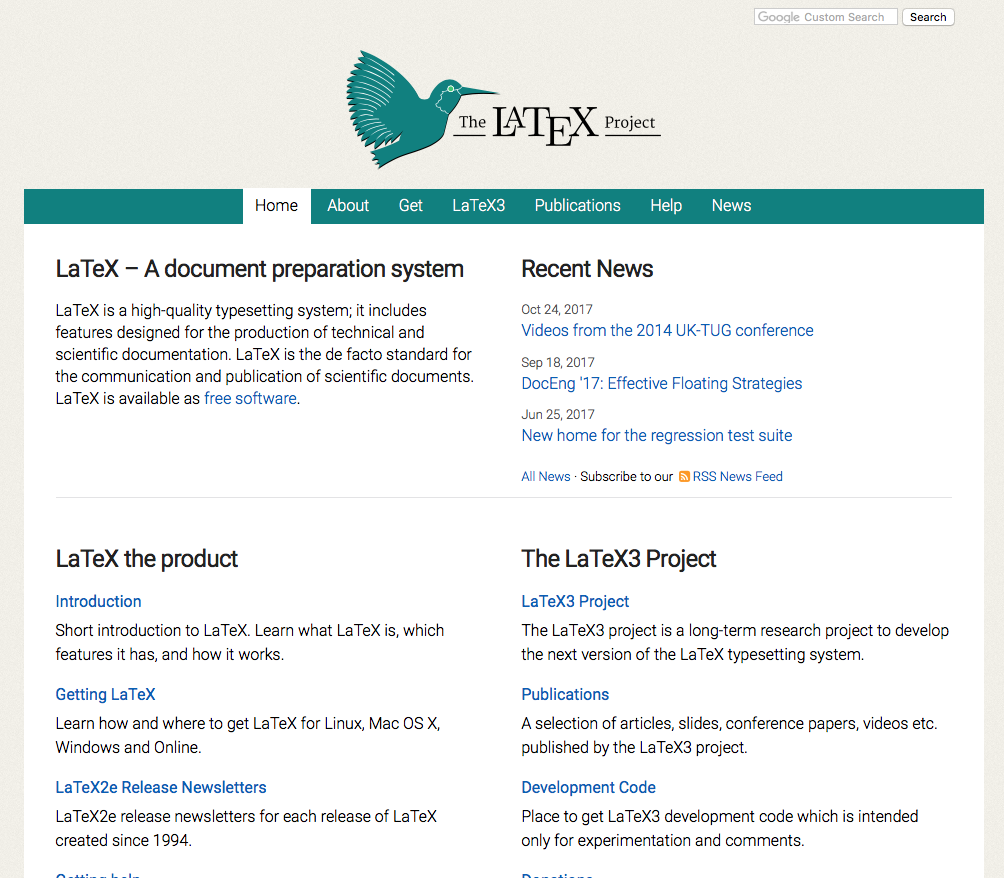
\includegraphics[width=0.7\textwidth]{figures/fig_latex_project_org}
\par\end{centering}

\caption{LaTeX Project}
\end{figure}


Puede obtener, en forma gratuita, las distribuciones de \LaTeX{},
según su plataforma, en:

\begin{description}
\item [Windows] \href{http://miktex.org/}{http://miktex.org/}; también puede
ocupar \href{http://www.tug.org/protext/}{http://www.tug.org/protext/}.

MikTex ofrece una versión básica. Después de instalarlo, asegúrese de descargar los paquetes adicionales requeridos para compilar esta plantilla.

\item [MacOS] \href{http://www.tug.org/mactex/}{http://www.tug.org/mactex/}.

La versión de MacTex es completa e incluye por defecto todos los paquetes necesarios para compilar esta plantilla.

\item [Unix/Linux] \href{http://www.tug.org/texlive/}{http://www.tug.org/texlive/}.

La instalación de TexLive en plataformas *nix es muy sencilla y directa a través de una consola (con permisos de administración):

(K/X)Ubuntu / Debian: \inlinecode{# apt-get install texlive}

Fedora: \inlinecode{# dnf install texlive}

RedHat / CentOS: \inlinecode{# yum install texlive}
\end{description}

Para una referencia completa sobre \LaTeX{}, recomendamos el libro
de \citealp{Lamport94}; aunque para solucionar problemas específicos,
su mejor aliado es Internet. Otros libros que puede consultar se presentan
en la Bibliografía \citep{Mittelbach04,Oetiker06,Roberts05}.


\section{Editores para \LaTeX}
Existen muchos editores de \LaTeX, la mayoría de ellos de distribución gratuita y con versiones para los distintos sistemas operativos:
\begin{description}
    \item [TexStudio] Mac, Windows y Linux. \href{www.texstudio.org}{www.texstudio.org}.
    \item [TexMaker] Mac, Windows y Linux.  \href{www.xm1math.net/texmaker/}{www.xm1math.net/texmaker/}.
    \item[TeXworks] Mac, Window y Linux. \href{https://www.tug.org/texworks/}{https://www.tug.org/texworks/}
    \item [TexShop] Mac. \href{http://pages.uoregon.edu/koch/texshop/}{http://pages.uoregon.edu/koch/texshop/}.
    \item[Kile] Linux y Mac (vía macports). \href{http://kile.sourceforge.net/}{http://kile.sourceforge.net/}.
    \item[LaTeXila] Linux y Mac (vía Homebrew). \href{https://wiki.gnome.org/Apps/LaTeXila\#Installation}{https://wiki.gnome.org/Apps/LaTeXila\#Installation}.
\end{description}

%...                    % Agregar aquí más capítulos


%%%%%%%%%%%%%%%%%%%%%%%%%%%%%%%%%%%%%
%	Bibliografía
%%%%%%%%%%%%%%%%%%%%%%%%%%%%%%%%%%%%%
\begin{spacing}{1}      % Single space for Bibliography
    \bibliographystyle{thesis_utfsm}    % Alternative 'apalike'
    \bibliography{bibliography}         % Archivo 'bibliography.bib'
\end{spacing}


%%%%%%%%%%%%%%%%%%%%%%%%%%%%%%%%%%%%%
%	Anexos (Opcional)
%%%%%%%%%%%%%%%%%%%%%%%%%%%%%%%%%%%%%
\appendix
%!TEX root = memoria.tex
\chapter{LICENCIA}\label{appx:licencia}

{\footnotesize
\verbatiminput{LICENSE} 
}

%...                  % Agregar más apéndices


\end{document}